\chapter{Optimal Fault-Tolerant Fixed-Time Control for Quadrotor UAV via Fuzzy Logic Approach}

\section{Introduction}
\label{sec:intro_ch4}

The increasing use of Unmanned Aerial Vehicles (UAVs) has reshaped numerous industries, leading to major progress across civilian, commercial, and military fields. Today, these platforms are essential for applications such as precision agriculture, disaster management, and complex autonomous surveillance \cite{UAV_rev, UAV_rev1, Ghamry2017}. Among the diverse array of aerial platforms, the quadcopter or quadrotor has emerged as one of the most widely adopted configurations in both academia and industry.  This prominent status is primarily attributed to its unique structural advantages, including mechanical simplicity, exceptional maneuverability in confined spaces, and robust Vertical Takeoff and Landing (VTOL) capabilities. By utilizing four fixed-pitch propellers to generate the requisite lift and control torques, the quadrotor elegantly eliminates the need for the complex, heavy swashplate mechanisms typically found in traditional helicopters, resulting in a highly agile and versatile aerial vehicle \cite{Bouabdallah2007}.

Despite its structural simplicity, the flight control of quadrotors presents a significant engineering challenge. The vehicle is inherently highly underactuated, possessing six degrees of freedom (DOF) but governed by only four independent control inputs. Consequently, its dynamic behavior is characterized by deeply coupled, highly nonlinear interactions between its rotational and translational states \cite{Underactuation1, RigidBody}. Furthermore, during real-world operations, quadrotors are exceptionally susceptible to exogenous wind disturbances and parametric uncertainties, such as fluctuating payloads or unmodeled aerodynamic drag \cite{ExternalDisturbances2}. Beyond these environmental factors, the most critical challenge to the operational viability of quadrotors is their severe vulnerability to physical faults. Failures such as the partial loss of rotor effectiveness or sudden sensor biases can drastically degrade flight performance, destabilize the underactuated dynamics, and rapidly lead to catastrophic crashes if not immediately mitigated \cite{Liu2022, Scognamiglio2024}.

To navigate these multifaceted control challenges, a broad spectrum of methodologies has been explored in the literature. Classical control techniques, such as PID and LQR, along with standard nonlinear approaches like Sliding Mode Control and Backstepping, have been widely implemented \cite{PID1, lqr1}. However, these conventional strategies heavily rely on exact mathematical models and inherently struggle to maintain robust performance in the presence of severe uncertainties. To enhance robustness, recent literature has increasingly combined intelligent approximators, such as Fuzzy Logic Systems or Neural Networks, to estimate unknown nonlinearities online \cite{fls}. Other approaches in the literature address the problem of physical hardware faults by employing either passive or active Fault-Tolerant Control (FTC) techniques, as extensively detailed in Chapter \ref{chp2} \cite{ftc_UAV_review1}. With all of that critical gap persists in the current state-of-the-art: traditional adaptive and fault-tolerant controllers typically guarantee only asymptotic or finite-time convergence. Under these paradigms, the system's recovery time is inextricably linked to its initial state at the exact moment a fault occurs \cite{Bhat2000}. For highly agile and underactuated quadrotors, there is an indispensable need for fast fault compensation and trajectory tracking convergence within a strict, pre-calculated short period that is completely independent of the initial conditions \cite{fxt, Zuo2018}. In this context, several recent works have addressed similar control challenges with different methodologies. In \cite{ranjan2025} proposed a fixed-time state observer-based adaptive neural fault-tolerant control scheme for quadrotor UAVs, wherein a sliding mode observer ensures fixed-time convergence of state estimation errors independent of initial conditions. While effective against actuator faults and external disturbances, this approach relies on neural networks for nonlinear function approximation and does not account for simultaneous sensor faults, nor does it incorporate any systematic parameter optimization strategy. Similarly, the work in\cite{robust_ftc_2024} introduced an adaptive fixed-time fault-tolerant control scheme combined with an Extended Kalman Filter (EKF) for online fault detection using an adaptive threshold technique. Although this method achieves fixed-time stability and avoids the need for known uncertainty bounds, it employs a discontinuous sliding mode control law that is inherently susceptible to the chattering phenomenon, which may compromise actuator longevity in practical UAV deployments. 

To explicitly address this critical gap, this chapter proposes a novel Optimal Fixed-Time Fault-Tolerant Adaptive Fuzzy Controller. The core of this architecture utilizes the recursive backstepping technique, rigorously enhanced with fixed-time stability theory to ensure deterministic convergence times. Unlike conventional models, this strategy deeply embeds Fuzzy Logic Systems (FLS) within the control loop to dynamically approximate and compensate for lumped uncertainties, exogenous disturbances, and simultaneous actuator and sensor faults online \cite{Wang1994}. Furthermore, recognizing that the efficacy of intelligent control heavily depends on precise parameter selection, a nature-inspired metaheuristic optimization algorithm specifically, the Whale Optimization Algorithm (WOA) is deployed \cite{woa}. The WOA systematically navigates the complex parameter space to optimally tune the controller gains, achieving a vital balance between stringent tracking precision and the minimization of excessive control effort.

The primary contributions are summarized as the establishment of a highly robust control framework capable of guaranteeing the  fixed-time stability of an underactuated quadrotor despite the simultaneous occurrence of severe actuator and sensor faults. By successfully integrating the WOA, this approach effectively overcomes the detrimental chattering phenomenon and prevents excessive actuator wear associated with aggressive high-frequency control signals, thereby ensuring smooth, energy-efficient, and robust trajectory tracking. The fundamental methodologies and core findings detailed in this chapter form the basis of our work published in the \textit{International Journal of Dynamics and Control} \cite{my2article}.

%The remainder of this chapter is organized as follows. Section \ref{sec:quad_dyn_model} establishes the comprehensive mathematical modeling of the quadrotor, incorporating the explicit formulation of actuator and sensor faults. Section \ref{sec:control_design_quadrotor} details the step-by-step design of the fixed-time adaptive fuzzy control law and provides rigorous stability proofs using Lyapunov theory. Subsequently, Section \ref{sec:optimization_setup} outlines the metaheuristic optimization setup utilizing the WOA. Finally, Section \ref{sec:sim_results_quadrotor} presents extensive comparative simulation validations to demonstrate the superiority of the proposed approach, followed by concluding remarks in Section \ref{sec:conclusion_ch4}.

\section{Dynamic Model and System Representation}
\label{sec:quad_dyn_model}

\begin{figure}
  \centerline{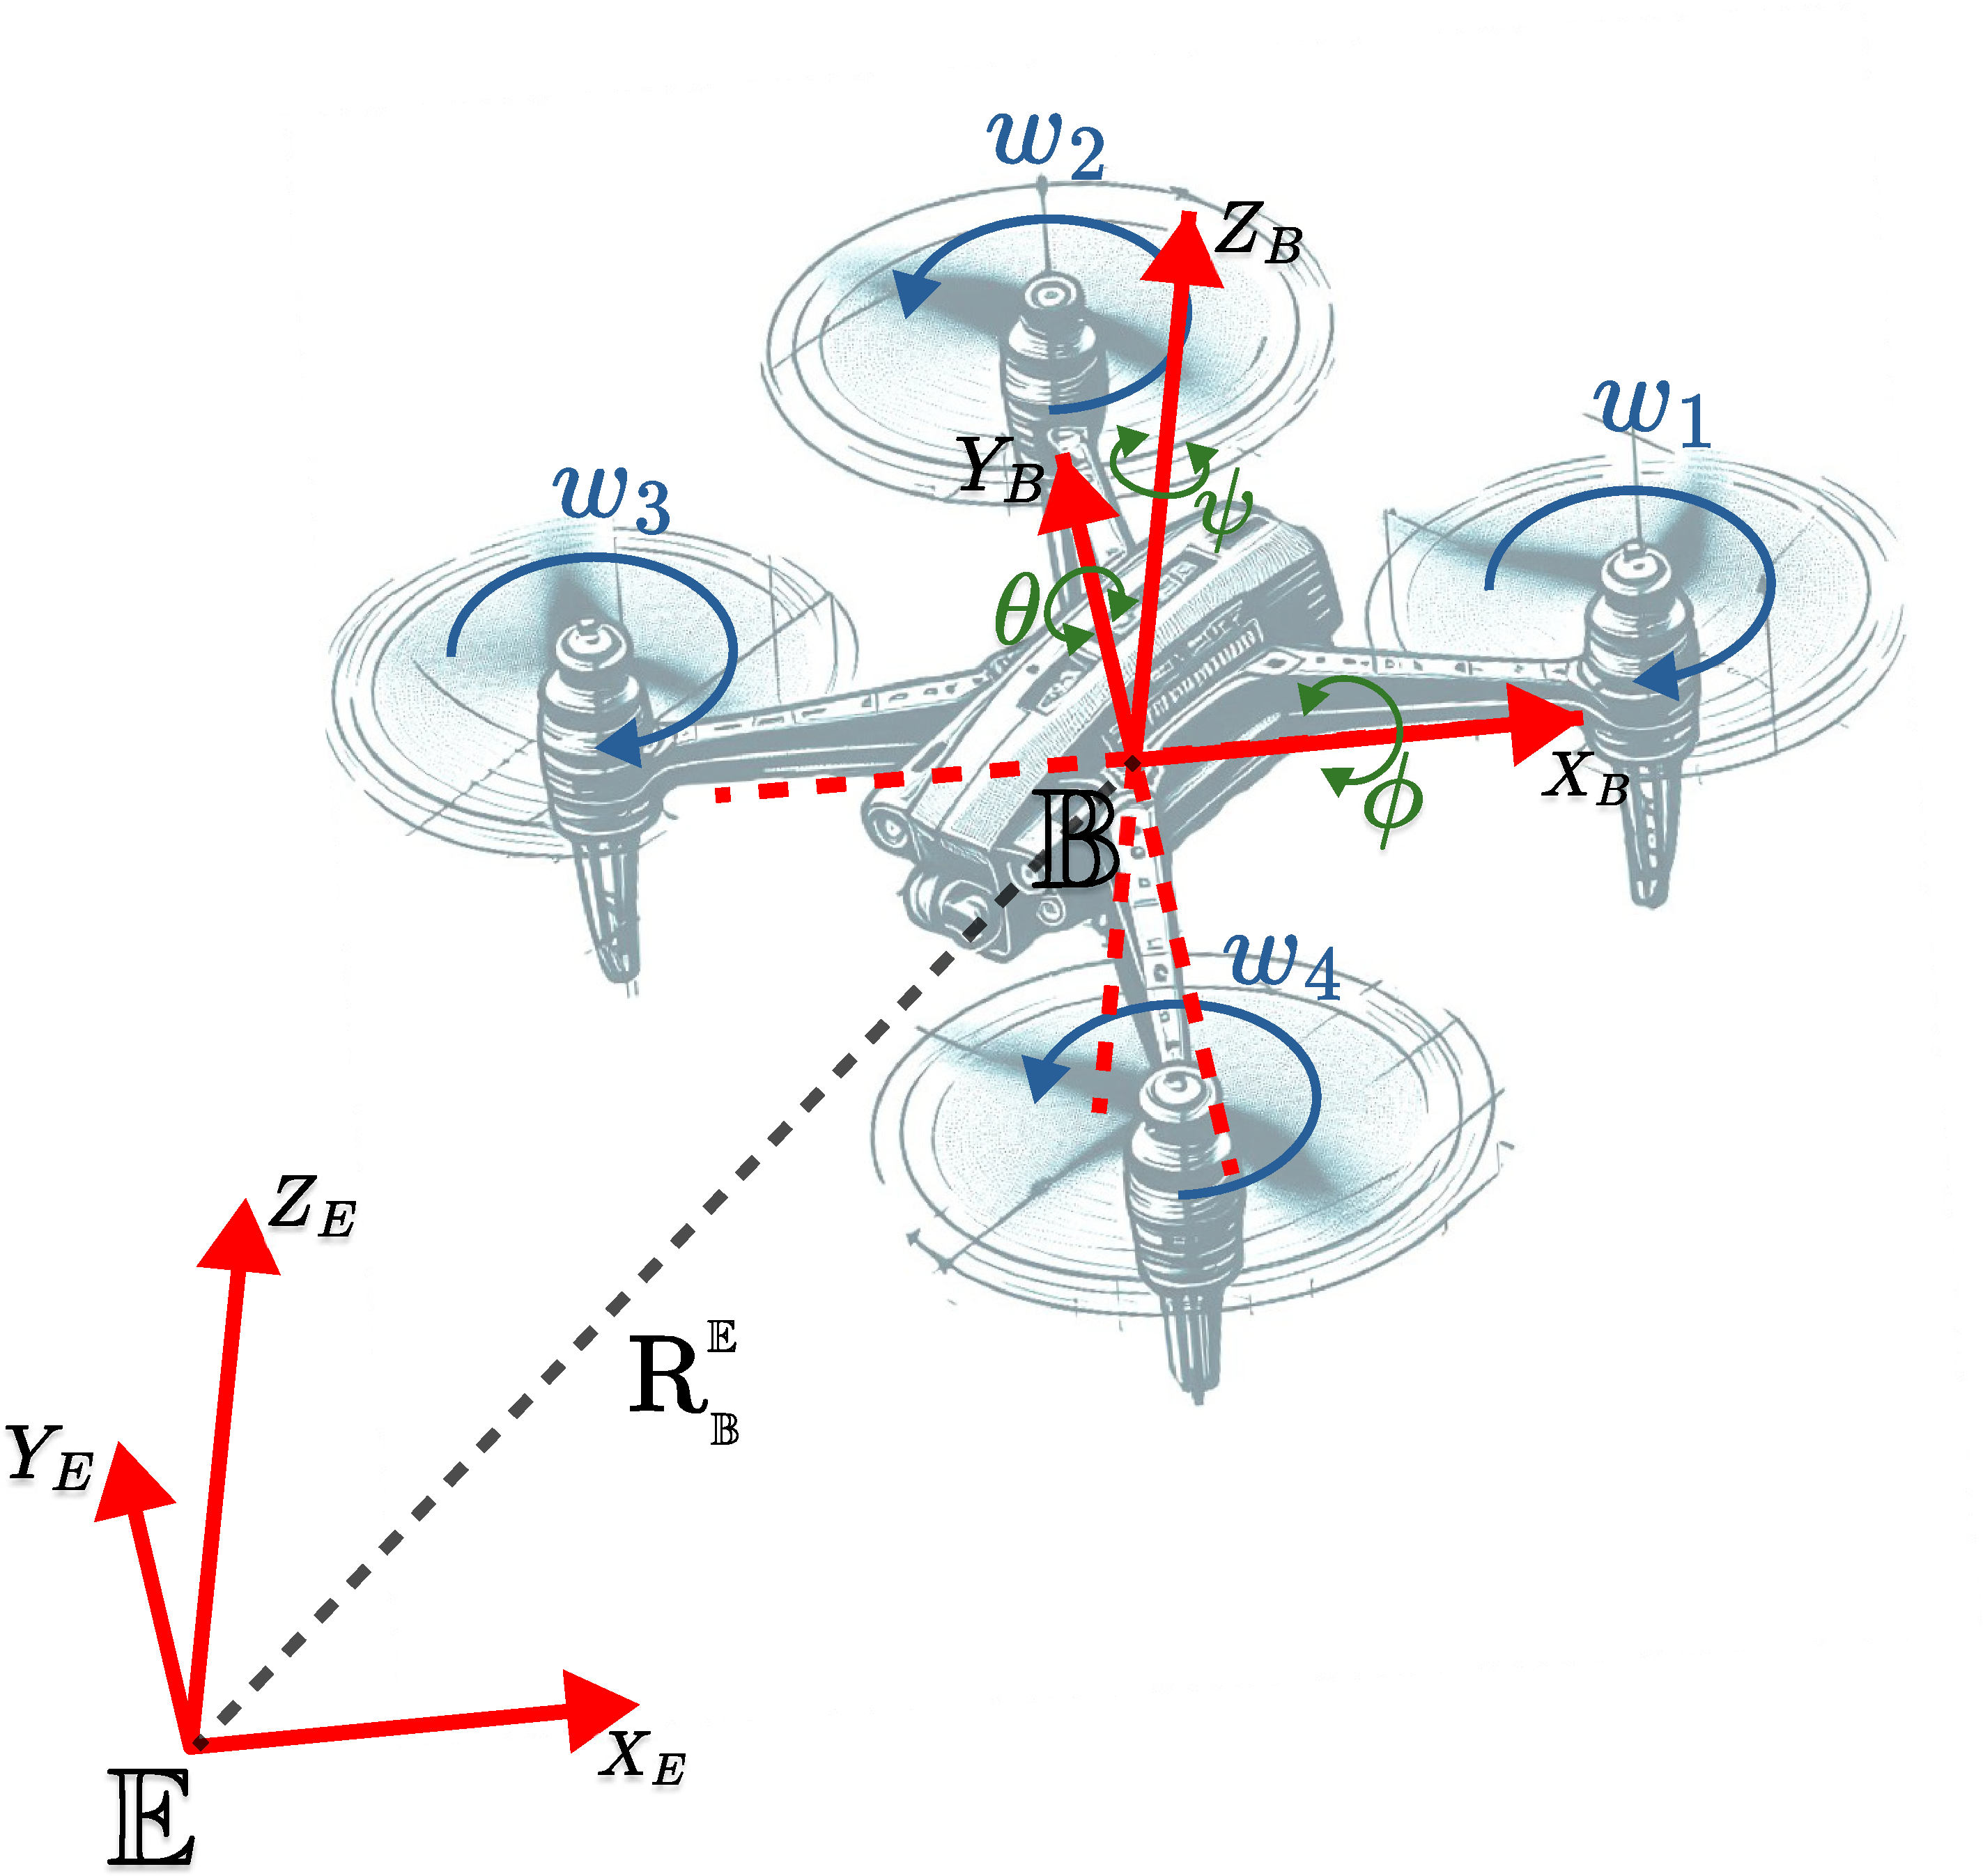
\includegraphics[width=8cm]{figure4/quad confg.pdf}}
  \caption{Schematic diagram of the quadrotor UAV showcasing rotor configuration and coordinate frames. }
  \label{quadrotor_configuration}
\end{figure}

This section details the mathematical model of the quadrotor UAV and formulates the system representation incorporating potential faults, which serves as the basis for the subsequent control system design.

\subsection{Mathematical Modeling of the Quadrotor}
A quadrotor is a type of UAV with six degrees of freedom (6-DOF) that navigates in three-dimensional space. Its motion is controlled by adjusting the angular velocities of its four rotors. Typically, two rotors spin clockwise and the other two spin counter-clockwise to maintain stability and control \cite{RigidBody}. The dynamics of the quadrotor are described using two coordinate frames, as depicted in Fig. \ref{quadrotor_configuration} \cite{ThrustDrag}.
The first is the Inertial Frame $\mathbb{E}(X_E, Y_E, Z_E)$, which is a fixed frame of reference typically aligned with the Earth's surface. The second is the Body-Fixed Frame $\mathbb{B}(X_B, Y_B, Z_B)$, a frame attached to the center of gravity (CG) of the quadrotor.

Let $\mathbf{p} = [p_x, p_y, p_z]^T$ be the position vector of the quadrotor's CG in the inertial frame $\mathbb{E}$. The orientation of the quadrotor is described by the Euler angles, contained in the attitude vector $\mathbf{W} = [\phi, \theta, \psi]^T$, representing roll, pitch, and yaw angles, respectively. The rotation matrix from the body-fixed frame $\mathbb{B}$ to the inertial frame $\mathbb{E}$, denoted as $\mathbf{R}_{\mathbb{B}}^{\mathbb{E}}$, is given by:
\begin{equation}
\label{eq:rotation_matrix_quad}
\mathbf{R}_{\mathbb{B}}^{\mathbb{E}} = 
\begin{bmatrix}
\cos\theta \cos\psi & \sin\phi \sin\theta \cos\psi - \cos\phi \sin\psi & \cos\phi \sin\theta \cos\psi + \sin\phi \sin\psi \\
\cos\theta \sin\psi & \sin\phi \sin\theta \sin\psi + \cos\phi \cos\psi & \cos\phi \sin\theta \sin\psi - \sin\phi \cos\psi \\
-\sin\theta & \sin\phi \cos\theta & \cos\phi \cos\theta
\end{bmatrix}
\end{equation}

The translational dynamics of the quadrotor are derived using the Newton-Euler formulation:
\begin{equation}
\label{eq:translational_dyn_quad}
m \ddot{\mathbf{p}} = m \mathbf{g}_I + \mathbf{R}_{\mathbb{B}}^{\mathbb{E}} \mathbf{T}_B
\end{equation}
where $m$ is the total mass of the quadrotor, $\mathbf{g}_I = [0, 0, -g]^T$ is the gravitational acceleration vector in $\mathbb{E}$, with $g$ being the gravitational constant and $\mathbf{T}_B = [0, 0, F_T]^T$ is the total thrust vector generated by the four rotors, acting along the $Z_B$-axis of the body frame. The total thrust magnitude $F_T$ is the sum of the forces produced by each rotor:
\begin{equation}
\label{eq:total_thrust_quad}
F_T = c_T \sum_{k=1}^{4} \omega_{k}^2
\end{equation}
where $c_T$ is the thrust coefficient and $\omega_{k}$ is the angular velocity of the $k$-th rotor.

The rotational dynamics in the body-fixed frame are given by:
\begin{equation}
\label{eq:rotational_dyn_quad}
\mathbf{J} \dot{\mathbf{\Omega}}_B = \mathbf{U}_{\tau} - \mathbf{\Omega}_B \times (\mathbf{J} \mathbf{\Omega}_B) + \mathbf{M}_{g}
\end{equation}
where $\mathbf{J} = \text{diag}(J_{xx}, J_{yy}, J_{zz})$ is the inertia matrix of the quadrotor, with $J_{xx}, J_{yy}, J_{zz}$ being the principal moments of inertia around the $X_B, Y_B, Z_B$ axes, respectively. $\mathbf{\Omega}_B = [\omega_x, \omega_y, \omega_z]^T$ is the angular velocity vector of the quadrotor in $\mathbb{B}$, with $\omega_x, \omega_y, \omega_z$ representing the roll, pitch, and yaw rates (approximated as $\dot{\phi}, \dot{\theta}, \dot{\psi}$ for small angles, or more generally related through a kinematic transformation). $\mathbf{U}_{\tau} = [\tau_{\phi}, \tau_{\theta}, \tau_{\psi}]^T$ is the control torque vector generated by the differential thrust of the rotors:
\begin{align}
\label{eq:control_torques_quad}
\tau_{\phi} &= L c_T (\omega_{2}^2 - \omega_{4}^2) \quad (\text{roll torque}) \\
\tau_{\theta} &= L c_T (\omega_{3}^2 - \omega_{1}^2) \quad (\text{pitch torque}) \\
\tau_{\psi} &= c_D (\omega_{1}^2 - \omega_{2}^2 + \omega_{3}^2 - \omega_{4}^2) \quad (\text{yaw torque})
\end{align}
Here, $L$ is the distance from the quadrotor's CG to the center of each rotor, and $c_D$ is the drag coefficient. $\mathbf{M}_{g}$ is the gyroscopic torque due to the rotation of the rotors, expressed as:
\begin{equation}
\label{eq:gyroscopic_torque_quad}
\mathbf{M}_{g} = \sum_{k=1}^{4} \mathbf{\Omega}_B \times J_r (\mathbf{\omega}_{k}^B \times \mathbf{I}_B (-1)^{k+1})
\end{equation}
where $J_r$ is the moment of inertia of a single rotor (assuming identical rotors), $\mathbf{\omega}_{k}^B = [0, 0, (-1)^{k+1}\omega_{k}]^T$ is the angular velocity of rotor $k$ relative to the body frame, and $\mathbf{I}_B = [0,0,1]^T$.
The model development relies on several common assumptions to ensure the model is both representative and mathematically tractable. First, the quadrotor's airframe is assumed to be a symmetric and rigid body, and its propellers are also considered rigid \cite{RigidBody}. Furthermore, the aerodynamic forces generated by the rotors, namely thrust and drag, are modeled to be proportional to the square of the rotor's angular speed \cite{ThrustDrag}. Lastly, to avoid kinematic singularities in the rotation matrix and ensure the system remains controllable, the Euler angles for roll ($\phi$) and pitch ($\theta$) are constrained to operate within the range of $-\pi/2 < \phi, \theta < \pi/2$.

Combining Eqs. \eqref{eq:translational_dyn_quad} and \eqref{eq:rotational_dyn_quad}, and expressing them in terms of Euler angle rates, the overall dynamic model of the quadrotor can be written as:
\begin{align}
\label{dynamic_eq}
\ddot{p}_x &= \frac{1}{m} (\cos\phi \sin\theta \cos\psi + \sin\phi \sin\psi) F_T \\
\ddot{p}_y &= \frac{1}{m} (\cos\phi \sin\theta \sin\psi - \sin\phi \cos\psi) F_T \\
\ddot{p}_z &= \frac{1}{m} (\cos\phi \cos\theta) F_T - g \\
\ddot{\phi} &= \frac{J_{yy}-J_{zz}}{J_{xx}} \dot{\theta}\dot{\psi} - \frac{1}{J_{xx}} \dot{\theta} \varpi J_r + \frac{1}{J_{xx}} \tau_{\phi} \\
\ddot{\theta} &= \frac{J_{zz}-J_{xx}}{J_{yy}} \dot{\phi}\dot{\psi} - \frac{1}{J_{yy}} \dot{\phi} \varpi J_r + \frac{1}{J_{yy}} \tau_{\theta} \\
\ddot{\psi} &= \frac{J_{xx}-J_{yy}}{J_{zz}} \dot{\phi}\dot{\theta} + \frac{1}{J_{zz}} \tau_{\psi}
\end{align}
These equations highlight the nonlinear and coupled nature of the quadrotor dynamics, where $\varpi = \omega_{1}^2 - \omega_{2}^2 + \omega_{3}^2 - \omega_{4}^2$. The system is underactuated, as there are six outputs ($p_x, p_y, p_z, \phi, \theta, \psi$) controlled by four inputs ($F_T, \tau_{\phi}, \tau_{\theta}, \tau_{\psi}$). To manage this, the horizontal positions ($p_x, p_y$) are typically controlled indirectly via desired roll ($\phi_d$) and pitch ($\theta_d$) angles, which are derived from virtual control inputs $V_x$ and $V_y$:
\begin{align}
\label{eq:virtual_inputs_quad}
V_x &= (\cos\phi \sin\theta \cos\psi + \sin\phi \sin\psi)F_T \\
V_y &= (\cos\phi \sin\theta \sin\psi - \sin\phi \cos\psi)F_T
\end{align}
From which, the desired roll and pitch angles can be computed as:
\begin{align}
\label{eq:desired_roll_pitch_quad}
\phi_d &= \arcsin\left(\frac{V_x \sin\psi_d - V_y \cos\psi_d}{F_T}\right) \\
\theta_d &= \arcsin\left(\frac{V_x \cos\psi_d + V_y \sin\psi_d}{F_T \cos\phi_d}\right)
\end{align}
where $V_x$ and $V_y$ are outputs of the position controller.

\subsection{Problem Formulation and System Representation with Faults}
From equations \eqref{dynamic_eq}, the quadrotor dynamics can be represented as a set of $j$ interconnected subsystems. For each subsystem $j \in \{p_x, p_y, p_z, \phi, \theta, \psi\}$, a second-order nominal model can be written in a compact form as:
\begin{equation}
\label{eq:compact_subsystem_quad_nominal}
\begin{cases}
\dot{\chi}_{j,1} = \chi_{j,2} \\
\dot{\chi}_{j,2} = f_j(\mathbf{x}) + g_j(\mathbf{x}) u_j + d_j(t) \\
y_j^m = h_j(\mathbf{x})
\end{cases}
\end{equation}
where $\chi_{j,1}$ represents the $j$-th position/angle state (e.g., $p_x, \phi$) and $\chi_{j,2}$ its derivative (e.g., $\dot{p}_x, \dot{\phi}$). $\mathbf{x}$ is the vector of all system states. $f_j(\mathbf{x})$ and $g_j(\mathbf{x})$ are nonlinear functions representing the system dynamics and control effectiveness, respectively. It's assumed that $0 < \underline{g}_j \le g_j(\mathbf{x}) \le \overline{g}_j$, where $\underline{g}_j$ and $\overline{g}_j$ are unknown positive constants. $u_j$ is the commanded control signal generated by the controller for the $j$-th subsystem. $d_j(t)$ represents time-varying external disturbances and unmodeled dynamics, assumed to be bounded such that $|d_j(t)| < \overline{d}_j$, with $\overline{d}_j$ being an unknown positive constant. The precise values of these bounds are not required for the controller development. $y_j^m$ is the measured output of the $j$-th subsystem via a function $h_j(\mathbf{x})$.

In practical scenarios, quadrotors are susceptible to sensor and actuator faults.

\textbf{Sensor Faults}:
Sensor measurements can be corrupted by faults. Consider two sensors for each subsystem providing measurements $y_{j,1}^s$ and $y_{j,2}^s$ (e.g., position and velocity, or angle and angular rate). These measurements are related to the true states $\chi_{j,1}$ and $\chi_{j,2}$ by:
\begin{equation}
\label{eq:sensor_fault_model_quad}
\begin{cases}
y_{j,1}^s(t) = \delta_{j,1}^M(t) \chi_{j,1}(t) + \delta_{j,1}^A(t) \\
y_{j,2}^s(t) = \delta_{j,2}^M(t) \chi_{j,2}(t) + \delta_{j,2}^A(t)
\end{cases}
\end{equation}

In this context, $\delta_{j,i}^M(t)$ represents the multiplicative sensor fault, which accounts for failures such as loss of effectiveness or gain variations. This term is bounded by $0 < \underline{\delta}_{j,i}^M \le \delta_{j,i}^M(t) \le 1$, where $\underline{\delta}_{j,i}^M$ denotes the lower bound of the sensor's effectiveness, ensuring the sensor retains some minimal functionality. Additionally, $\delta_{j,i}^A(t)$ represents the additive sensor fault, capturing errors like bias or drift. This fault is assumed to be bounded such that $|\delta_{j,i}^A(t)| \le \overline{\delta}_{j,i}^A$, where $\overline{\delta}_{j,i}^A$ signifies the unknown upper bound of the additive fault magnitude.

\textbf{Actuator Faults}:
The actual control input $u_{j,a}$ delivered by an actuator can differ from the commanded control signal $u_j$ due to faults. This is modeled as:
\begin{equation}
\label{eq:actuator_fault_model_quad}
u_{j,a}(t) = \delta_{A,j}^M(t) u_j(t) + \delta_{A,j}^A(t)
\end{equation}
Similarly, regarding the actuator dynamics, $\delta_{A,j}^M(t)$ denotes the multiplicative actuator fault, characterizing phenomena such as loss of effectiveness or power degradation. This factor is constrained by $0 < \underline{\delta}_{A,j}^M \le \delta_{A,j}^M(t) \le 1$, where $\underline{\delta}_{A,j}^M$ represents the lower bound of actuator efficiency. Furthermore, $\delta_{A,j}^A(t)$ signifies the additive actuator fault, corresponding to issues like bias. This term satisfies $|\delta_{A,j}^A(t)| \le \overline{\delta}_{A,j}^A$, where $\overline{\delta}_{A,j}^A$ indicates the unknown upper limit of the additive fault's magnitude. Collectively, these faults directly degrade the generated thrust and torques, significantly impacting the quadrotor's dynamic behavior.

\textbf{System Representation with Faults}:
Considering the sensor measurements $y_{j,1}^s, y_{j,2}^s$ and the faulty actuator output $u_{j,a}$, the dynamics of the $j$-th subsystem in terms of these measured/actual values become:
\begin{equation}
\label{eq:faulty_subsystem_dyn_quad}
\begin{cases}
\dot{y}_{j,1}^s = \dot{\delta}_{j,1}^M \chi_{j,1} + \delta_{j,1}^M \chi_{j,2} + \dot{\delta}_{j,1}^A \\
\dot{y}_{j,2}^s = \dot{\delta}_{j,2}^M \chi_{j,2} + \delta_{j,2}^M [f_j(\mathbf{x}) + g_j(\mathbf{x})(\delta_{A,j}^M u_j + \delta_{A,j}^A) + d_j(t)] + \dot{\delta}_{j,2}^A
\end{cases}
\end{equation}
This system representation incorporates unknown nonlinear dynamics $f_j, g_j$, external disturbances $d_j(t)$, and faults in both sensors ($\delta_{j,i}^M, \delta_{j,i}^A$) and actuators ($\delta_{A,j}^M, \delta_{A,j}^A$). The control objective is to design a robust fault-tolerant control law for $u_j$ such that the system outputs ($p_x, p_y, p_z, \phi, \theta, \psi$) accurately track their desired reference trajectories $\chi_{j,d}$, ensuring fixed-time stability for the closed-loop system despite these faults and uncertainties.

\section{Control Design and Stability Analysis}
\label{sec:control_design_quadrotor}

This section outlines the design of the Optimal Fault-Tolerant Adaptive Fuzzy Control (OFTAFC) strategy for the quadrotor UAV. The primary goal is to develop a robust control law that guarantees fixed-time trajectory tracking despite unknown nonlinear dynamics, external disturbances, and the presence of both sensor and actuator faults. The controller design leverages the backstepping technique, augmented by adaptive fuzzy logic systems (FLS) for online estimation of unknown functions and a metaheuristic optimization algorithm, the Whale Optimization Algorithm (WOA), for optimal parameter tuning. The overall architecture of the proposed control scheme is illustrated in Fig.~\ref{fig:quadrotor_control_architecture}.

\begin{figure}[h!]
    \centering
    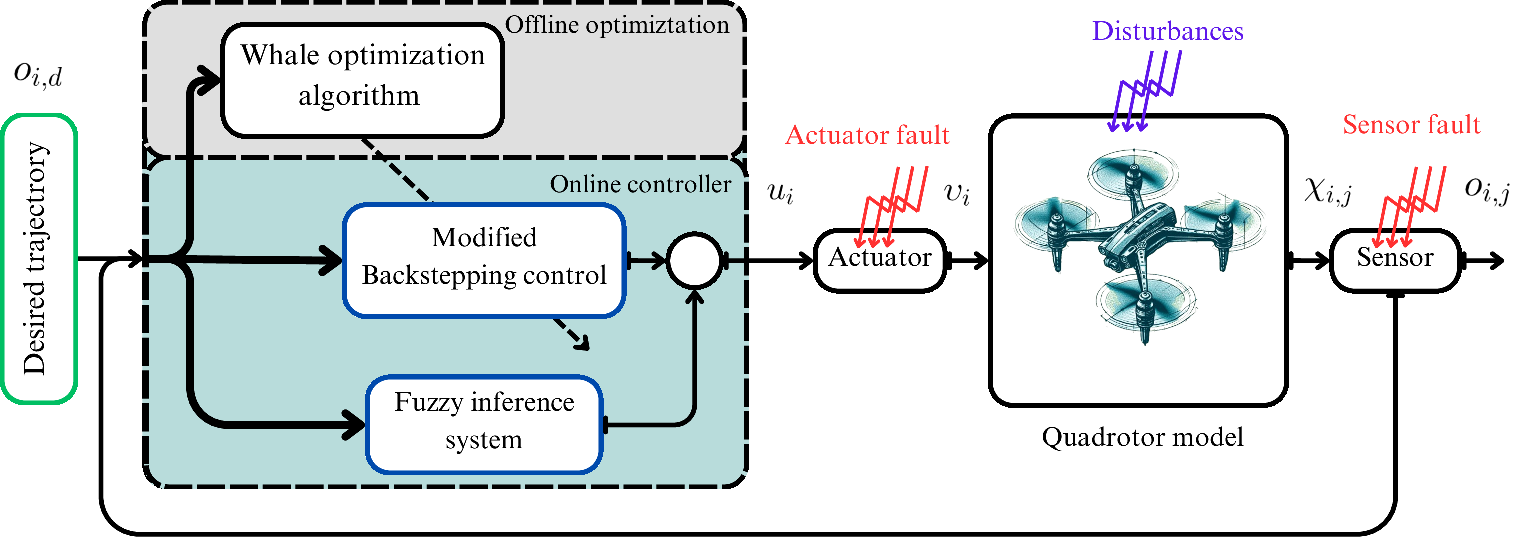
\includegraphics[width=14cm]{figure4/schema.pdf}
    \caption{Block diagram of the proposed fault-tolerant fixed-time fuzzy controller architecture for the quadrotor UAV. \label{fig:quadrotor_control_architecture}}
\end{figure}

The design procedure follows a systematic backstepping approach for each of the six interconnected subsystems $j \in \{p_x, p_y, p_z, \phi, \theta, \psi\}$. The system dynamics for each subsystem are considered in the form of Eq. \eqref{eq:faulty_subsystem_dyn_quad}, which incorporates sensor and actuator faults.

\subsection{Step 1: Position/Angle Tracking Control}
We begin by defining the tracking errors for each subsystem $j$:
\begin{align}
    e_{j,1} &= y_{j,1}^s - \chi_{j,d} \label{eq:error_e_j1} \\
    e_{j,2} &= y_{j,2}^s - \alpha_{j,1} \label{eq:error_e_j2}
\end{align}
where $y_{j,1}^s$ and $y_{j,2}^s$ are the measured (potentially faulty) states, $\chi_{j,d}$ is the desired reference trajectory, and $\alpha_{j,1}$ is a virtual control law to be designed in this step.

The time derivative of the first error term $e_{j,1}$ is obtained from Eq.~\eqref{eq:error_e_j1} and the faulty system representation in Eq. \eqref{eq:faulty_subsystem_dyn_quad}:
\begin{align}
    \dot{e}_{j,1} &= \dot{y}_{j,1}^s - \dot{\chi}_{j,d} \nonumber \\
    &= \left( \dot{\delta}_{j,1}^M \chi_{j,1} + \delta_{j,1}^M \chi_{j,2} + \dot{\delta}_{j,1}^A \right) - \dot{\chi}_{j,d} \label{eq:e_j1_dot_raw}
\end{align}
Substituting $\chi_{j,2} = (y_{j,2}^s - \delta_{j,2}^A) / \delta_{j,2}^M = (e_{j,2} + \alpha_{j,1} - \delta_{j,2}^A) / \delta_{j,2}^M$ into the above equation, we can write $\dot{e}_{j,1}$ in terms of $e_{j,2}$ and the virtual control $\alpha_{j,1}$, along with unknown nonlinearities and fault terms. 

\begin{equation}
    \dot{e}_{j,1} = \dot{\delta}_{j,1}^M \chi_{j,1} + \frac{\delta_{j,1}^M}{\delta_{j,2}^M}  (e_{j,2} + \alpha_{j,1} - \delta_{j,2}^A)  + \dot{\delta}_{j,1}^A - \dot{\chi}_{j,d}
\end{equation}


Let's group these unknown terms into a function, we call it $\mathcal{F}_{j,1}(\mathbf{x})$, that  implicitly includes all unknown dynamics and fault components affecting the first error dynamics, such that it can be approximated by an FLS.

Consider the first Lyapunov function candidate for each subsystem $j$:
\begin{equation}
    \mathcal{L}_{j,1} = \frac{1}{2} e_{j,1}^2 + \frac{1}{2\kappa_{j,1}} \tilde{W}_{j,1}^2 \label{eq:lyapunov_Vj1}
\end{equation}
where $\kappa_{j,1}$ is a positive design constant, and $\tilde{W}_{j,1} = W_{j,1} - \hat{W}_{j,1}$ is the estimation error for the ideal weight vector $W_{j,1}$ of the FLS.

The time derivative of $\mathcal{L}_{j,1}$ is:
\begin{align}
    \dot{\mathcal{L}}_{j,1} &= e_{j,1} \dot{e}_{j,1} + \frac{1}{\kappa_{j,1}} \tilde{W}_{j,1} \dot{\tilde{W}}_{j,1} \nonumber \\
    &= e_{j,1} \left[ \dot{\delta}_{j,1}^M \chi_{j,1} + \frac{\delta_{j,1}^M}{\delta_{j,2}^M}  (e_{j,2} + \alpha_{j,1} - \delta_{j,2}^A)  + \dot{\delta}_{j,1}^A - \dot{\chi}_{j,d} \right] - \frac{1}{\kappa_{j,1}} \tilde{W}_{j,1} \dot{\hat{W}}_{j,1} \label{eq:Vj1_dot_expanded}
\end{align}

using Lemma \ref{lemma3} and defining  $h_{j,1}$ as the upper bound of $\frac{\delta_{j,1}^M}{\delta_{j,2}^M}$ we can obtain

\begin{equation}
\label{eq:dL_j1_rewritten}
\begin{aligned}
\dot{\mathcal{L}}_{j,1} &\leq e_{j,1} \left[ \dot{\delta}_{j,1}^M \chi_{j,1} + \frac{\delta_{j,1}^M}{\delta_{j,2}^M}( \alpha_{j,1} - \delta_{j,2}^A) + \frac{1}{2}h_{j,1}^2 e_{j,1} \right. \\
& \left. + \frac{1}{2}e_{j,1} - \dot{\chi}_{j,d} \right] + \frac{1}{2}e_{j,2}^2 + \frac{1}{2} (\overline{\delta}_{j,1}^A)^2 - \frac{1}{\kappa_{j,1}}\tilde{W}_{j,1}\dot{\hat{W}}_{j,1}
\end{aligned}
\end{equation}

Lets define the following function:
\begin{equation}\label{eq:F_j1_def}
\mathcal{F}_{j,1}(\mathbf{S}_{j,1}) = \dot{\delta}_{j,1}^M \chi_{j,1} - \frac{\delta_{j,1}^M}{\delta_{j,2}^M}\alpha_{j,1} + \frac{1}{2}h_{j,1}^2 e_{j,1} + e_{j,1} - \dot{\chi}_{j,d},
\end{equation}
where $\mathbf{S}_{j,1}$ is the input vector of the used fuzzy systems. Then, the dynamics of $\dot{\mathcal{L}}_{j,1}$ become
\begin{equation} \label{eq:dL_j1_f}
\begin{aligned}
\dot{\mathcal{L}}_{j,1} &\leq  e_{j,1}\left (\mathcal{F}_{j,1}(\mathbf{S}_{j,1}) + \frac{\delta_{j,1}^M}{\delta_{j,2}^M}\alpha_{j,1} - \frac{1}{2}e_{j,1}\right ) \\
&+ \frac{1}{2}e_{j,2}^2 + \frac{1}{2} (\overline{\delta}_{j,i}^A)^2 - \frac{1}{\kappa_{j,1}}\tilde{W}_{j,1}\dot{\hat{W}}_{j,1}.
\end{aligned}
\end{equation}
According to Eq. \eqref{eq:fls_approx}, the nonlinear function $\mathcal{F}_{j,1}(\mathbf{S}_{j,1})$ can be approximated using the FLS as:
\begin{equation}
\mathcal{F}_{j,1}(\mathbf{S}_{j,1}) = \mathbf{\Theta}_{j,1}^T\mathbf{\Psi}_{j,1}(\mathbf{S}_{j,1}) + \zeta_{j,1}(\mathbf{S}_{j,1}).
\end{equation}
From equation \eqref{eq:F_j1_def} and using Young's inequality, we can obtain
\begin{equation}\label{eq:Youngs_step1}
\begin{aligned}
e_{j,1}\mathcal{F}_{j,1}(\mathbf{S}_{j,1}) &\leq \frac{\overline{\delta}_{j,1}^M}{2\lambda_{j,1}}e_{j,1}^2W_{j,1}\mathbf{\Psi}_{j,1}^T(\mathbf{S}_{j,1})\mathbf{\Psi}_{j,1}(\mathbf{S}_{j,1}) + \frac{\lambda_{j,1}}{2\overline{\delta}_{j,1}^M} + \frac{1}{2}e_{j,1}^2 + \frac{1}{2}\epsilon_{j,1}^2,
\end{aligned}
\end{equation}
where $W_{j,1} = ||\Theta_{j,1}||^2$, $\lambda_{j,1}$ is a positive constant, and the fuzzy logic inputs are $\mathbf{S}_{j,1}=[\chi_{j,1} \ \chi_{j,d} \ \dot{\chi}_{j,d}]^T$. Substituting equation \eqref{eq:Youngs_step1} into \eqref{eq:dL_j1_f} gives
\begin{equation}\label{eq:dL_j1_subbed}
\begin{aligned}
\dot{\mathcal{L}}_{j,1} &\leq e_{j,1}\left( \frac{\overline{\delta}_{j,1}^M}{2\lambda_{j,1}}e_{j,1}W_{j,1}\mathbf{\Psi}_{j,1}^T(\mathbf{S}_{j,1})\mathbf{\Psi}_{j,1}(\mathbf{S}_{j,1}) + \frac{\delta_{j,1}^M}{\delta_{j,2}^M}\alpha_{j,1} - \frac{1}{2}e_{j,1}\right ) \\
&+ \frac{\lambda_{j,1}}{2\overline{\delta}_{j,1}^M} + \frac{1}{2}e_{j,1}^2 + \frac{1}{2}\epsilon_{j,1}^2 + \frac{1}{2}e_{j,2}^2 - \frac{\overline{\delta}_{j,1}^M}{\kappa_{j,1}}\tilde{W}_{j,1}\dot{\hat{W}}_{j,1}.
\end{aligned}
\end{equation}
Then, the virtual control inputs can be designed as
\begin{equation} \label{eq:alpha_j1}
\alpha_{j,1} = -\overline{\mathcal{A}}_{j,1}\tanh \left (\frac{e_{j,1}\overline{\mathcal{A}}_{j,1}}{\eta_{j,1}}\right ),
\end{equation}
with,
\begin{equation} \label{eq:A_bar_j1}
\overline{\mathcal{A}}_{j,1} = k_{j,1}e_{j,1}^{2\rho_1 - 1} + \beta_{j,1}e_{j,1}^{2\rho_2 - 1} + \frac{1}{2\lambda_{j,1}}e_{j,1}\hat{W}_{j,1}\mathbf{\Psi}_{j,1}^T(\mathbf{S}_{j,1})\mathbf{\Psi}_{j,1}(\mathbf{S}_{j,1}).
\end{equation}
According to Lemma 3, we can obtain the following inequality:
\begin{equation}\label{eq:tanh_inequality}
\begin{aligned}
e_{j,1}\frac{\delta_{j,1}^M}{\delta_{j,2}^M}\alpha_{j,1} &\leq -e_{j,1}\overline{\delta}_{j,1}^M\overline{\mathcal{A}}_{j,1} + 0.2785\overline{\delta}_{j,1}^M\eta_{j,1}.
\end{aligned}
\end{equation}
The adaptation law is introduced as
\begin{equation}\label{eq:theta_hat_dot_j1}
\dot{\widehat{W}}_{j,1} = \kappa_{j,1}(\frac{1}{2\lambda_{j,1}}e_{j,1}^2\mathbf{\Psi}_{j,1}^T(\mathbf{S}_{j,1})\mathbf{\Psi}_{j,1}(\mathbf{S}_{j,1}) - \sigma_{j,1}\hat{W}_{j,1}).
\end{equation}
Substituting equations \eqref{eq:tanh_inequality} and \eqref{eq:theta_hat_dot_j1} into \eqref{eq:dL_j1_subbed}, we obtain

\begin{equation}\label{eq:dL_j1_final}
\dot{\mathcal{L}}_{j,1} \leq \overline{\delta}_{j,1}^M(-k_{j,1}e_{j,1}^{2\rho_{1}} - \beta_{j,1}e_{j,1}^{2\rho_{2}}) + \overline{\delta}_{j,1}^M\sigma_{j,1}\tilde{W}_{j,1}\hat{W}_{j,1} + \frac{1}{2}e_{j,2}^{2} + \mathcal{B}_{j,1},
\end{equation}

\begin{equation} \label{eq:h_j1}
\mathcal{B}_{j,1} = 0.2785\overline{\delta}_{j,1}^M\eta_{j,1} + \frac{\lambda_{j,1}}{2\overline{\delta}_{j,1}^M} + \epsilon_{j,1}^{2}.
\end{equation}

\subsection{Step 2: Actuator Control Input Design}
Now, consider the derivative of the second error term $e_{j,2}$ from Eq.~\eqref{eq:error_e_j2}:
\begin{align}
    \dot{e}_{j,2} &= \dot{y}_{j,2}^s - \dot{\alpha}_{j,1} \nonumber \\
    &=  \dot{\delta}_{j,2}^M \chi_{j,2} + \delta_{j,2}^M \left[ f_j(\mathbf{x}) + g_j(\mathbf{x}) \left( \delta_{A,j}^M u_j + \delta_{A,j}^A \right) + d_j(t) \right] + \dot{\delta}_{j,2}^A  - \dot{\alpha}_{j,1} \label{eq:e_j2_dot_raw}
\end{align}
Similar to Step 1, we group all unknown nonlinear terms, disturbances, and fault components into a new unknown function $\mathcal{F}_{j,2}(\mathbf{x})$, and introduce $e_{j,1}$ into this step to simplify the total Lyapunov function:
\begin{equation}
    \mathcal{L}_{j,2} = \mathcal{L}_{j,1} + \frac{1}{2} e_{j,2}^2 + \frac{1}{2\kappa_{j,2}} \tilde{W}_{j,2}^2 \label{eq:lyapunov_Vj2}
\end{equation}
where $\kappa_{j,2}$ is a positive design constant, and $\tilde{W}_{j,2} = W_{j,2} - \hat{W}_{j,2}$ is the estimation error for the ideal weight vector $W_{j,2}$ of the FLS.

The time derivative of $\mathcal{L}_{j,2}$ is:
\begin{align}
    \dot{\mathcal{L}}_{j,2} &= \dot{\mathcal{L}}_{j,1} + e_{j,2} \dot{e}_{j,2} - \frac{1}{\kappa_{j,2}} \tilde{W}_{j,2} \dot{\hat{W}}_{j,2} \nonumber \\
    &= \left( -k_{j,1} e_{j,1}^{2\rho_1} - \beta_{j,1} e_{j,1}^{2\rho_2} + e_{j,1} e_{j,2} + \sigma_{j,1} \tilde{W}_{j,1} \hat{W}_{j,1} + \mathcal{F}_{j,1} \right. \nonumber \\
    &\quad \left. + e_{j,2} (e_{j,1} + u_j + \mathcal{F}_{j,2}(\mathbf{x})) - \frac{1}{\kappa_{j,2}} \tilde{W}_{j,2} \dot{\hat{W}}_{j,2} \right) \label{eq:Vj2_dot_expanded}
\end{align}

\begin{equation} \label{eq:dL_j2_subbed}
\begin{aligned}
\dot{\mathcal{L}}_{j,2} &\leq \overline{\delta}_{j,1}^M \left(-k_{j,1}e_{j,1}^{2\rho_{1}} - \beta_{j,1}e_{j,1}^{2\rho_{2}}\right) + \overline{\delta}_{j,1}^M \sigma_{j,1}\tilde{W}_{j,1}\hat{W}_{j,1} + \frac{1}{2}e_{j,2}^{2} + \mathcal{B}_{j,1} + \\
&e_{j,2}\left[\dot{\delta}_{j,2}^M \chi_{j,2} + \delta_{j,2}^M \left[f_j(\mathbf{x}) + g_j(\mathbf{x})\left(\delta_{A,j}^M u_j + \delta_{A,j}^A\right) + d_j(t)\right] - \dot{\alpha}_{j,1}\right] + \\
& \frac{1}{2}e_{j,2}^{2} + \frac{1}{2}\epsilon_{j,2}^{2} - \frac{\overline{\Omega}_{j}}{\kappa_{j,2}}\tilde{W}_{j,2}\dot{\hat{W}}_{j,2}.
\end{aligned}
\end{equation}

Define the following function
\begin{equation} \label{eq:F_j2_def}
\mathcal{F}_{j,2}\left(\mathbf{S}_{j,2}\right) = \dot{\delta}_{j,2}^M \chi_{j,2} + \delta_{j,2}^M f_j(\mathbf{x}) + \delta_{j,2}^M g_j(\mathbf{x})\delta_{A,j}^A - \dot{\alpha}_{j,1} + 2e_{j,2}^{2}
\end{equation}

Using the FLS definition, the approximation of $\mathcal{F}_{j,2}(\mathbf{S}_{j,2})$ can be introduced as
\begin{equation} 
\mathcal{F}_{j,2}\left(\mathbf{S}_{j,2}\right) = \mathbf{W}_{j,2}^{T}\mathbf{\Psi}_{j,2}\left(\mathbf{S}_{j,2}\right) + \zeta_{j,2}(\mathbf{S}_{j,2}).
\end{equation}

From equation \eqref{eq:F_j2_def} and using Young's inequality, we can obtain
\begin{equation} \label{eq:Youngs_step2_full}
e_{j,2}\mathcal{F}_{j,2}\left(\mathbf{S}_{j,2}\right) \leq \frac{1}{2\lambda_{j,2}}e_{j,2}^{2}W_{j,2}\mathbf{\Psi}_{j,2}^{T}\left(\mathbf{S}_{j,2}\right)\mathbf{\Psi}_{j,2}\left(\mathbf{S}_{j,2}\right) +\frac{\lambda_{j,2}}{2\overline{\Omega}_{j}} + \frac{1}{2}e_{j,2}^{2} + \frac{1}{2}\epsilon_{j,2}^{2},
\end{equation}

Now, we can design the actual fixed-time controller as
\begin{equation} \label{eq:u_j_tanh}
u_{j} = -\overline{\mathcal{A}}_{j,2}\tanh\left(\frac{e_{j,2}\overline{\mathcal{A}}_{j,2}}{\eta_{j,2}}\right),
\end{equation}
with
\begin{equation} \label{eq:A_bar_j2_def}
\overline{\mathcal{A}}_{j,2} = k_{j,2}e_{j,2}^{2\rho_{1} - 1} + \beta_{j,2}e_{j,2}^{2\rho_{2} - 1} + \frac{1}{2\lambda_{j,2}}e_{j,2}\hat{W}_{j,2}\mathbf{\Psi}_{j,2}^{T}\left(\mathbf{S}_{j,2}\right)\mathbf{\Psi}_{j,2}\left(\mathbf{S}_{j,2}\right).
\end{equation}

The adaptation law is constructed as follows: 
\begin{equation} \label{eq:theta_hat_dot_j2} \dot{\widehat{W}}{j,2} = \kappa{j,2}\left(\frac{1}{2\lambda_{j,2}}e_{j,2}^{2}\mathbf{\Psi}{j,2}^{T}\left(\mathbf{S}{j,2}\right)\mathbf{\Psi}{j,2}\left(\mathbf{S}{j,2}\right) - \sigma_{j,2}\hat{W}{j,2}\right). 
\end{equation}
Substituting equations \eqref{eq:u_j_tanh} and \eqref{eq:theta_hat_dot_j2} into \eqref{eq:dL_j2_subbed}, one can obtain 

\begin{equation} \label{eq:dL_j2_final_expanded} 
\begin{aligned} \dot{\mathcal{L}}_{j,2} &\leq \overline{\delta}_{j,1}^M\left(-k_{j,1}e_{j,1}^{2\rho_{1}} - \beta_{j,1}e_{j,1}^{2\rho_{2}}\right) + \overline{\delta}_{j,1}^M\sigma_{j,1}\tilde{W}_{j,1}\hat{W}_{j,1} - \\ & \left(k_{j,2}e_{j,2}^{2\rho_{1}} + \beta_{j,2}e_{j,2}^{2\rho_{2}}\right) + \overline{\Omega}_{j}\sigma_{j,2}\tilde{W}_{j,2}\hat{W}_{j,2} + \mathcal{B}_{j,2}, 
\end{aligned} 
\end{equation} 

\begin{equation} \label{eq:h_j2} \mathcal{B}_{j,2} = \mathcal{B}_{j,1} + 0.2785\overline{\Omega}_{j}\eta_{j,2} + \frac{\lambda_{j,2}}{2\overline{\Omega}_{j}} + \epsilon_{j,2}^{2}. 
\end{equation}



\subsection{Stability Analysis}
\label{sec:stability_analysis_quadrotor}

The stability of the entire closed-loop system is formally established by demonstrating its practical fixed-time stability.

\textbf{Theorem 1:} Consider the closed-loop system of the quadrotor UAV described by Eq.~\eqref{eq:faulty_subsystem_dyn_quad}, with the designed virtual control law in Eq.~\eqref{eq:alpha_j1}, the actual control law in Eq.~\eqref{eq:u_j_tanh}, and the adaptive laws in Eqs.~\eqref{eq:theta_hat_dot_j1} and \eqref{eq:theta_hat_dot_j2}. Under appropriate selection of positive design parameters $k_{j,1}, \beta_{j,1}, k_{j,2}, \beta_{j,2}, \kappa_{j,1}, \kappa_{j,2}$ and given the properties of fuzzy logic systems and fixed-time stability lemmas, the practical fixed-time stability of the quadrotor system is guaranteed. The system states will converge to a compact set around the equilibrium point within a fixed settling time that is independent of the initial conditions.

\textbf{Proof:}
To analyze the stability of the entire multi-subsystem quadrotor, we define a global Lyapunov function $\mathcal{L} = \sum_{j \in \{p_x, \dots, \psi\}} \mathcal{L}_{j,2}$. The time derivative of this global Lyapunov function can be expressed by summing the individual $\dot{\mathcal{L}}_{j,2}$ terms from Eq.~\eqref{eq:dL_j2_final_expanded}. By applying the inequality $\sigma \tilde{W} \hat{W} \le -\frac{\sigma}{2} \tilde{W}^2 + \frac{\sigma}{2} W^2$ and combining similar terms, the overall derivative of $\mathcal{L}$ can be shown to satisfy the conditions of Lemma 2 of the source paper. Specifically, $\dot{\mathcal{L}}$ can be upper bounded by:
\begin{equation}
    \dot{\mathcal{L}} \le -\alpha \mathcal{L}^p - \beta \mathcal{L}^q + \eta \label{eq:global_lyapunov_form}
\end{equation}
where $\alpha, \beta > 0$, $p > 1$, $0 < q < 1$, and $\eta$ is a positive bounded constant. The specific values of $\alpha, \beta, p, q,$ and $\eta$ are derived from the chosen controller parameters and the bounds of the approximation errors.
According to Lemma 2, this form guarantees that the system states converge to a compact residual set around the equilibrium point within a fixed settling time $T_{\max}$. This settling time is independent of the initial conditions, which is a crucial advantage for safety-critical UAV applications. The size of the residual set and the settling time are directly influenced by the values of $\eta, \alpha, \beta, p, q$. By careful selection of the design parameters, the value of $\eta$ can be made arbitrarily small, ensuring the states converge arbitrarily close to the equilibrium point. The detailed algebraic steps and proofs for this form are consistent with similar fixed-time control schemes found in the literature.

\subsection{Optimization of Control Parameters}
\label{sec:optimization_setup}

The proposed fault-tolerant adaptive fuzzy controller is governed by a rich set of design parameters. These include the fixed-time exponents $\rho_1$ and $\rho_2$, the FLS learning rates $\kappa_{j,1}$ and $\kappa_{j,2}$, the inequality constants $\lambda_{j,1}$ and $\lambda_{j,2}$, the hyperbolic tangent smoothing coefficients $\eta_{j,1}$ and $\eta_{j,2}$, and the $\sigma$-modification leakage terms $\xi_{j,1}$ and $\xi_{j,2}$. Among this full parameter set, the backstepping gains $k_{j,1}$, $\beta_{j,1}$, $k_{j,2}$, and $\beta_{j,2}$ exert the most significant and direct influence on the closed-loop performance. These gains simultaneously govern the rate of convergence of the tracking errors, the aggressiveness of the control action, and the system's ability to reject faults and disturbances within the required fixed time. Selecting these four gains manually is an exceptionally complex task, given the highly underactuated, nonlinear, and strongly coupled dynamics of the quadrotor and the six interconnected subsystems that must be optimized jointly. Therefore, the Whale Optimization Algorithm (WOA) is employed for their automatic and systematic selection, as extensively detailed in Chapter~\ref{chp2}.

\begin{figure}[htbp]
    \centering
    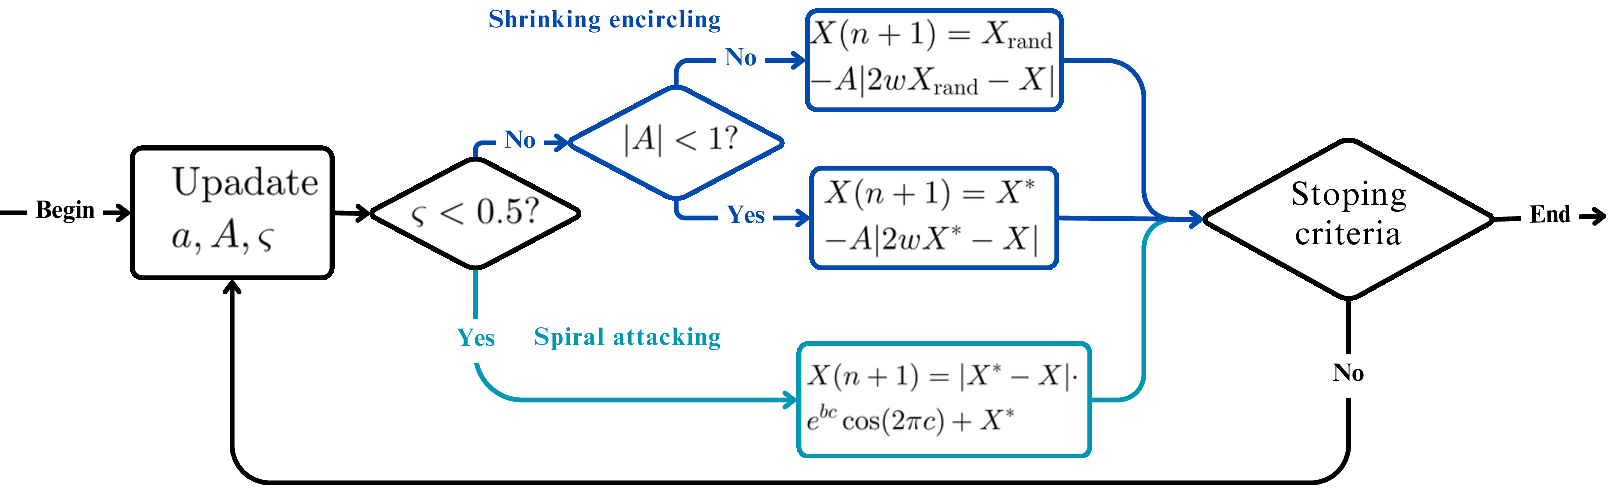
\includegraphics[width=14cm]{figure4/flowchart.pdf} 
    \caption{Flowchart of the WOA optimization process for quadrotor controller tuning.}
    \label{fig:woa_optimization}
\end{figure}

The WOA, inspired by the bubble-net hunting strategy of humpback whales, is a highly efficient nature-inspired metaheuristic that navigates the parameter search space through a probabilistic combination of shrinking encircling, spiral updating, and random exploration mechanisms, making it particularly effective at escaping local optima in high-dimensional problems. The optimization procedure adopted in this work is illustrated in Fig.~\ref{fig:woa_optimization}. The algorithm is run for 100 iterations with a population of 50 search agents (simulated whales). The optimization is conducted separately for the position subsystems and the attitude subsystems, using the following global objective functions:
\begin{equation}
    J_j = \sqrt{\frac{1}{N} \sum_{k=1}^{N} e_{j,1}^2(k)} + \lambda \int_{0}^{T_{\text{sim}}} \left| \frac{dv_j(t)}{dt} \right| dt
    \label{eq:global_cost_function_quad}
\end{equation}
The first term is the Root Mean Square Error (RMSE) over $N$ discrete samples, penalizing trajectory tracking inaccuracy. The second term is the Integral of the Absolute Derivative of the control input, penalizing high-frequency actuation and promoting signal smoothness to reduce mechanical wear on the quadrotor's rotors. The weighting factor $\lambda$ is set to $0.3$ to maintain an appropriate balance between tracking precision and actuator smoothness. The search for the four gains is constrained within the bounds $0 \leq k_{j,1}, \beta_{j,1}, k_{j,2}, \beta_{j,2} \leq 20$ to ensure physically realizable and practically stable control actions. At each iteration, the search behavior is governed by the coefficient $a$, which decreases linearly from $2$ to $0$, progressively transitioning the algorithm from global exploration toward local exploitation. The choice between the shrinking encircling mechanism and the spiral attacking movement is determined by a switching probability $\varsigma = 0.5$, while the spiral trajectory is parameterized by a random number $c$ drawn uniformly from $[-1, 1]$. The transition between exploration and exploitation phases is further controlled by the magnitude of the coefficient vector $\vec{A}$: when $|\vec{A}| < 1$, the algorithm exploits the current best solution, whereas when $|\vec{A}| \geq 1$, it performs a global random search. The optimized values of these gains, along with the complete set of remaining controller parameters, are reported in the simulation section.

\section{Simulation Results and Discussion}
\label{sec:sim_results_quadrotor}

This section evaluates the performance of the proposed optimal fault-tolerant adaptive
fuzzy control strategy for a quadrotor UAV. Simulations were conducted to assess the
controller's effectiveness in tracking a predefined trajectory while contending with
external disturbances, as well as combined sensor and actuator faults. The quadrotor
model parameters used are consistent with those in \cite{passive1}. The desired
reference trajectory for the quadrotor is defined as follows:
\begin{equation}
    p_{x_d}(t) =
    \begin{cases}
        0 & 0 \leq t < 5\,\text{s} \\
        \cos\!\left(\dfrac{\pi}{10}t\right) & 5\,\text{s} \leq t < 40\,\text{s}
    \end{cases}
\end{equation}
\begin{equation}
    p_{y_d}(t) =
    \begin{cases}
        0 & 0 \leq t < 5\,\text{s} \\
        \sin\!\left(\dfrac{\pi}{10}t\right) & 5\,\text{s} \leq t < 40\,\text{s}
    \end{cases}
\end{equation}
\begin{equation}
    p_{z_d}(t) =
    \begin{cases}
        0.5t & 0 \leq t < 5\,\text{s} \\
        4    & 5\,\text{s} \leq t < 40\,\text{s}
    \end{cases}
\end{equation}
\begin{equation}
    \psi_d(t) =
    \begin{cases}
        0 & 0 \leq t < 5\,\text{s} \\
        \dfrac{\pi}{40}t & 5\,\text{s} \leq t < 40\,\text{s}
    \end{cases}
\end{equation}
This trajectory involves an initial vertical ascent, followed by a circular motion
in the horizontal plane while maintaining altitude and continuously changing yaw angle.
The remaining controller parameters were fixed as follows: $\gamma_{j,1} = \gamma_{j,2} = 0.5$,
$\mu_{j,1} = \mu_{j,2} = 0.1$, $\eta_{j,1} = \eta_{j,2} = 0.001$, $\rho_1 = \tfrac{3}{2}$,
and $\rho_2 = \tfrac{3}{4}$. The two Fuzzy Logic Systems (FLS) employed as adaptive
estimators for each subsystem utilize Gaussian membership functions to cover the
input space of each fuzzy system. The backstepping gains $k_{j,1}$, $\beta_{j,1}$,
$k_{j,2}$, and $\beta_{j,2}$, which exert the most significant and direct influence on
the closed-loop convergence rate, tracking accuracy, and fault rejection capability,
were optimized offline via the WOA algorithm. The optimized values are listed in
Table~\ref{tab:WOA_parameters}. The simulations encompass two main scenarios: performance
evaluation under external disturbances, and performance evaluation under combined
sensor and actuator faults. These scenarios are designed to thoroughly test the proposed
Fault-Tolerant Fixed-Time Adaptive Fuzzy Controller (FTFxTAFC) and to benchmark
it against a conventional PID controller and a non-optimized version of the proposed
controller.

\begin{table}[htbp]
\centering
\caption{Optimal control gains obtained via WOA.}
\label{tab:WOA_parameters}
\begin{tabular}{@{}lcccc@{}}
\toprule
\textbf{Subsystem} & $k_{j,1}$ & $\beta_{j,1}$ & $k_{j,2}$ & $\beta_{j,2}$ \\ \midrule
Position: $x,\,y$  & $15.301$ & $1.303$ & $3.290$ & $1.635$ \\ \midrule
Position: $z$      & $2.185$  & $1.475$ & $3.320$ & $8.513$ \\ \midrule
Attitude: $\varphi,\,\theta$ & $4.015$ & $7.701$ & $7.440$ & $0.982$ \\ \midrule
Attitude: $\psi$   & $1.611$  & $6.311$ & $3.337$ & $17.126$ \\
\bottomrule
\end{tabular}
\end{table}

\subsection{Performance Evaluation under External Disturbances}

In the first scenario, the controller's robustness was tested against significant external disturbances affecting both the translational and rotational dynamics of the quadrotor. These disturbances, designed to simulate realistic environmental conditions such as wind gusts, are depicted in Fig.~\ref{disturbances}.

\begin{figure}[h!]
    \centering
    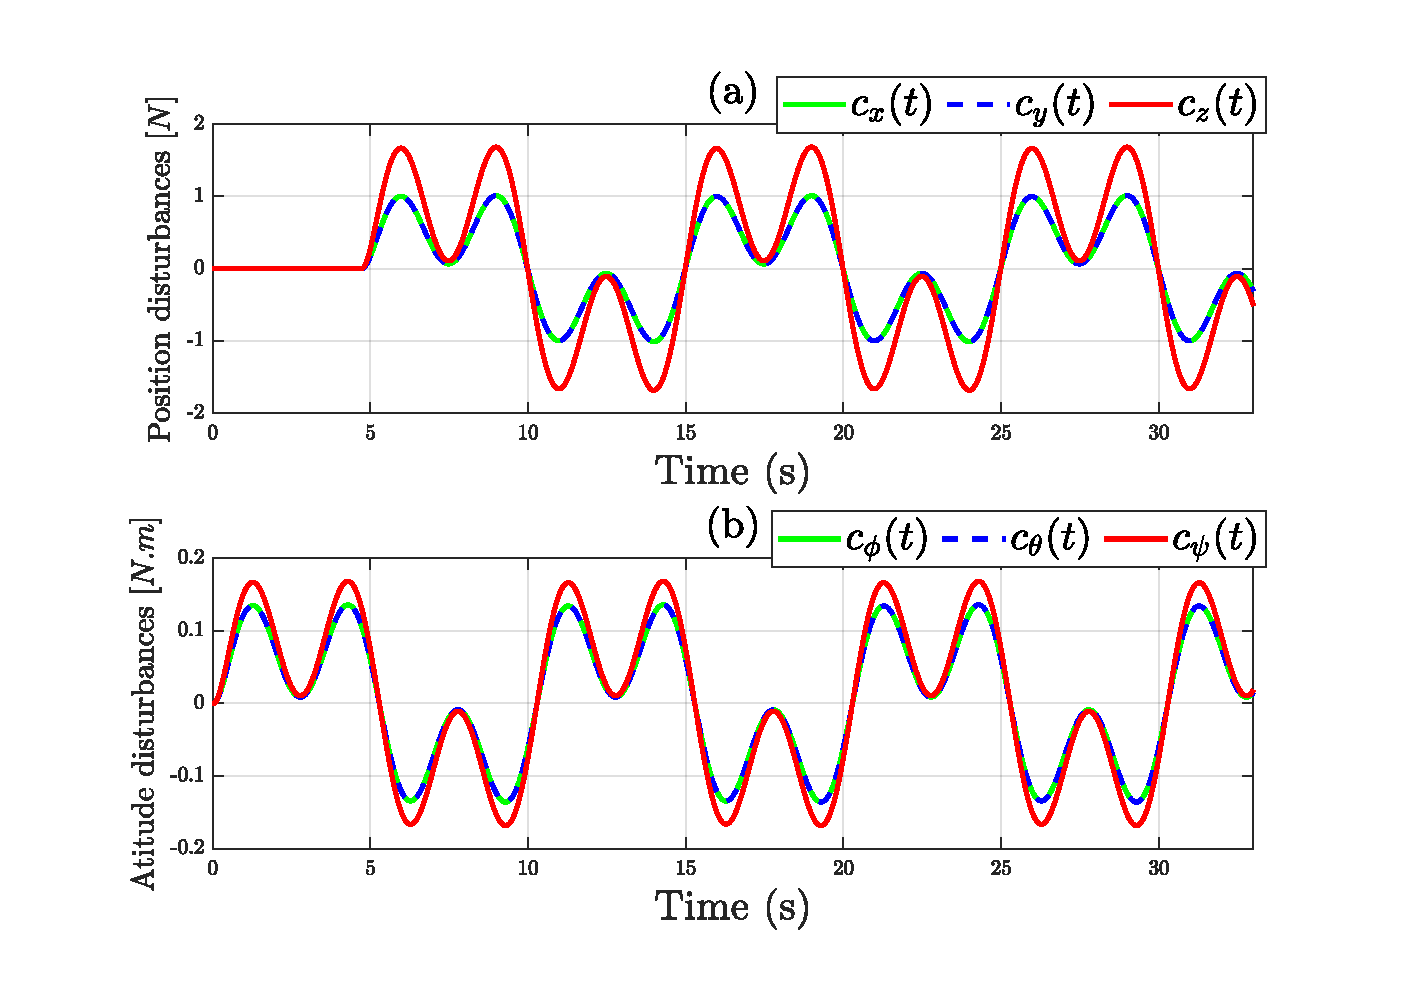
\includegraphics[width=14cm]{figure4/disturbances.pdf}
    \caption{Profiles of external disturbances applied to the quadrotor UAV: (a) translational disturbances, (b) rotational disturbances. }
    \label{disturbances}
\end{figure}

The attitude tracking performance of the optimized proposed controller under these disturbances is illustrated in Fig.~\ref{attitudeWithDisturbances}. The roll ($\phi$), pitch ($\theta$), and yaw ($\psi$) angles demonstrate accurate tracking of their desired references, with smooth transitions and minimal deviation despite the substantial disturbances. This highlights the controller's ability to effectively reject external perturbations and maintain attitude stability.

\begin{figure}[h!]
    \centering
    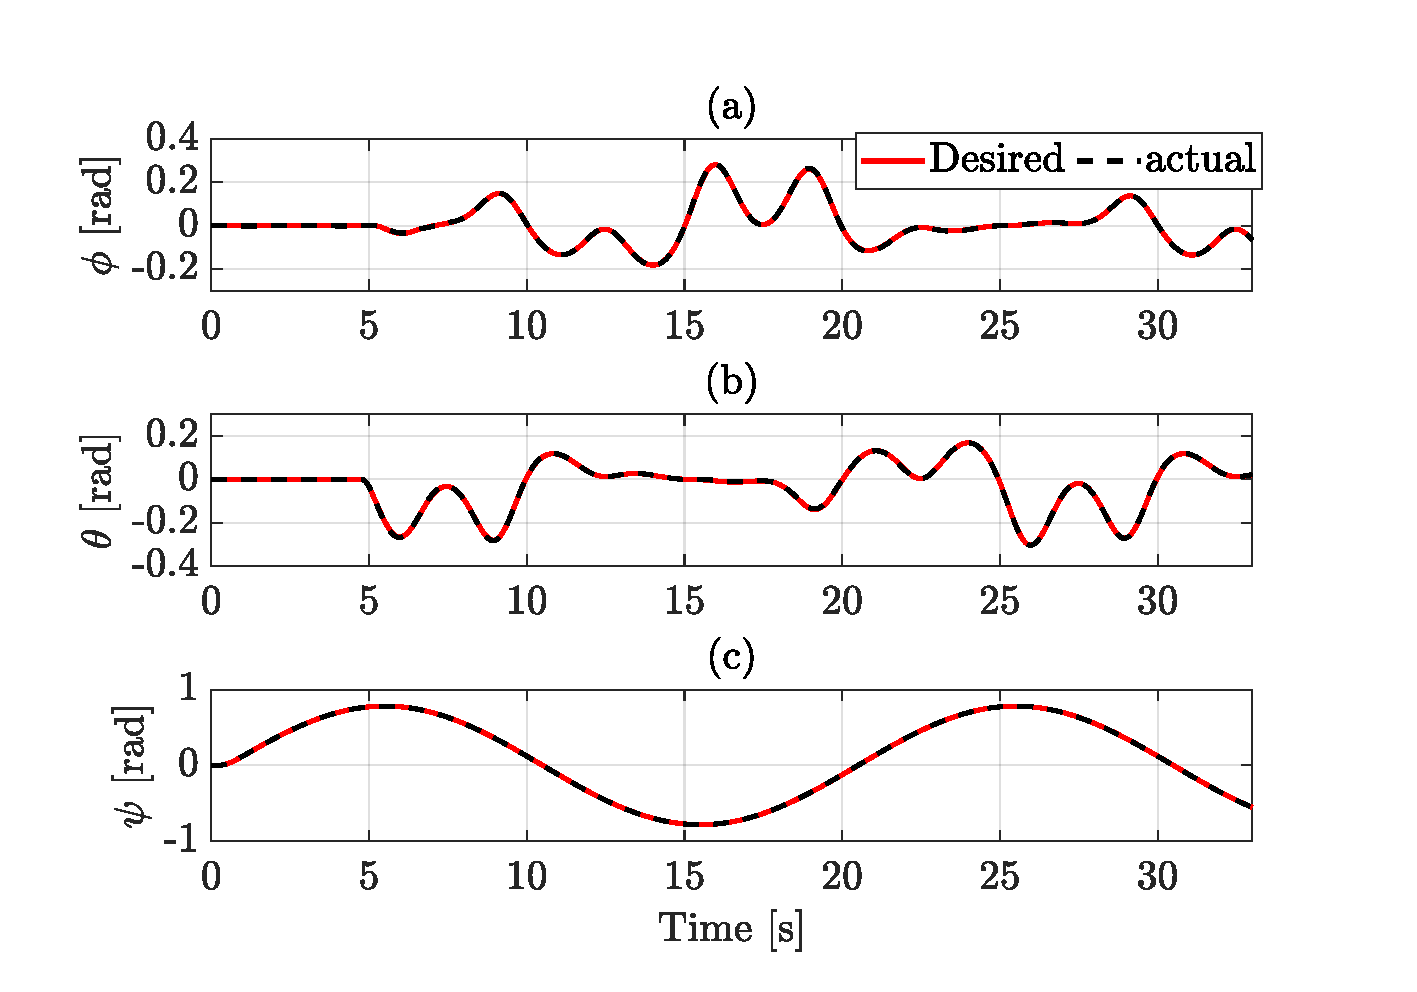
\includegraphics[width=14cm]{figure4/attitudeWithDisturbances.pdf}
    \caption{Attitude tracking performance under external disturbances for: (a) roll ($\phi$), (b) pitch ($\theta$), and (c) yaw ($\psi$) angles. }
    \label{attitudeWithDisturbances}
\end{figure}

Fig.~\ref{3dDisturbances} presents a comparative 3D trajectory tracking performance among three control strategies: a conventional PID controller (Set1), the proposed fault-tolerant fuzzy controller with parameters tuned via trial-and-error (Set2), and the proposed controller with WOA-optimized parameters (Set3). The PID controller (Set1) exhibits significant deviations and oscillatory behavior, struggling with the system's nonlinearities and the imposed disturbances. The non-optimized proposed controller (Set2) shows improved performance over PID but still presents noticeable tracking errors, particularly during more dynamic phases of the trajectory. In contrast, the WOA-optimized controller (Set3) achieves superior tracking accuracy, with its path closely adhering to the desired trajectory in both side and top-down views. These results underscore the significant benefit of the WOA-based optimization in enhancing the controller's tracking capabilities.

\begin{figure}[h!]
    \centering
    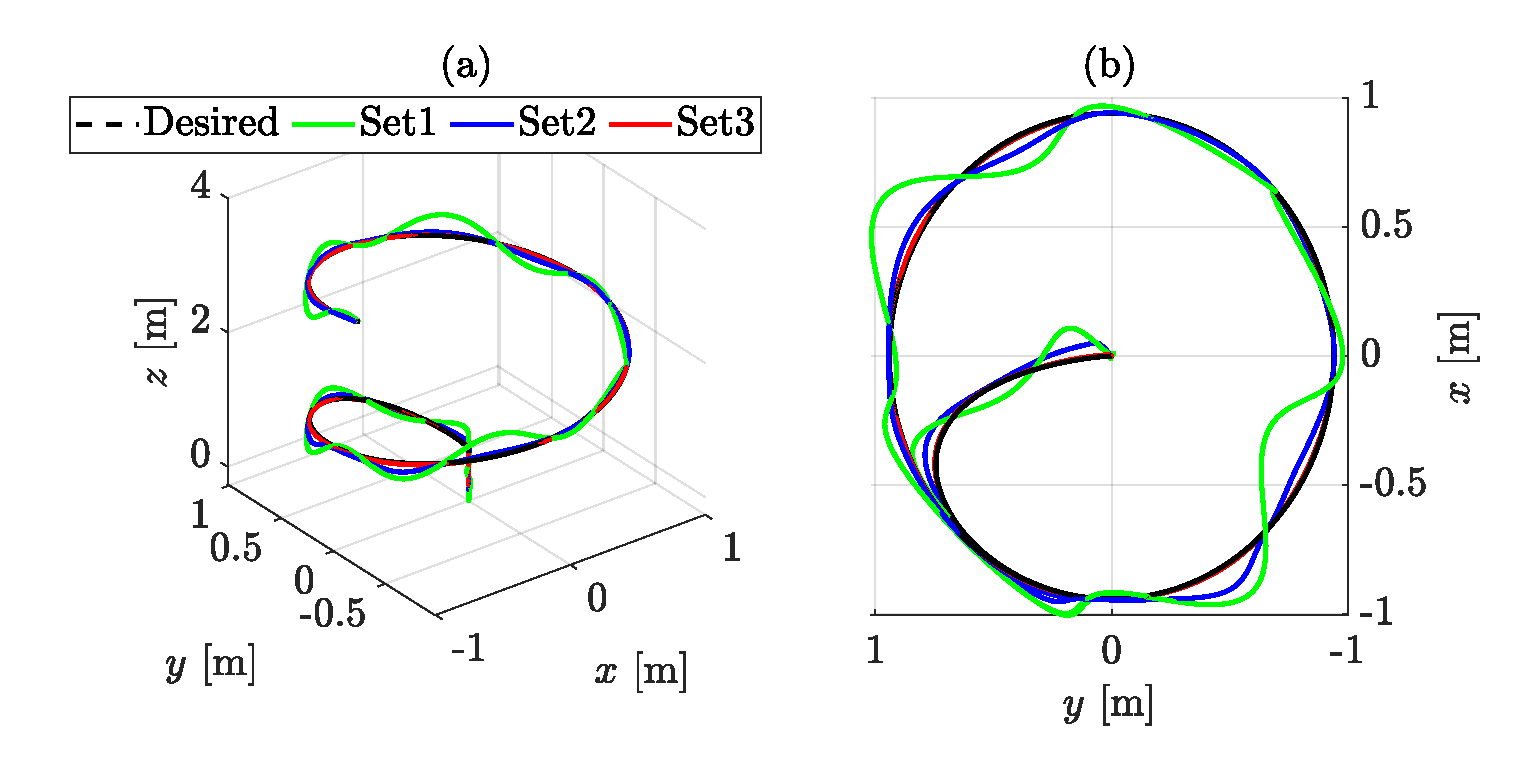
\includegraphics[width=14cm]{figure4/3dDisturbances.pdf}
    \caption{3D trajectory tracking comparison under disturbances between PID, trial-based, and WOA-optimized controllers: (a) side view, (b) top-down view. }
    \label{3dDisturbances}
\end{figure}

The control inputs generated by the optimized controller during this disturbance scenario are shown in Fig.~\ref{inputDisturbances}. The angular torques ($\tau_\phi, \tau_\theta, \tau_\psi$) remain within reasonable bounds (approximately $\pm0.2 \, N \cdot m$), indicating an efficient control effort in counteracting the disturbances. The total thrust force ($F_T$) displays smooth variations, adjusting appropriately to maintain altitude control and stability amidst the perturbations, reaching up to approximately $6N$.

\begin{figure}[h!]
    \centering
    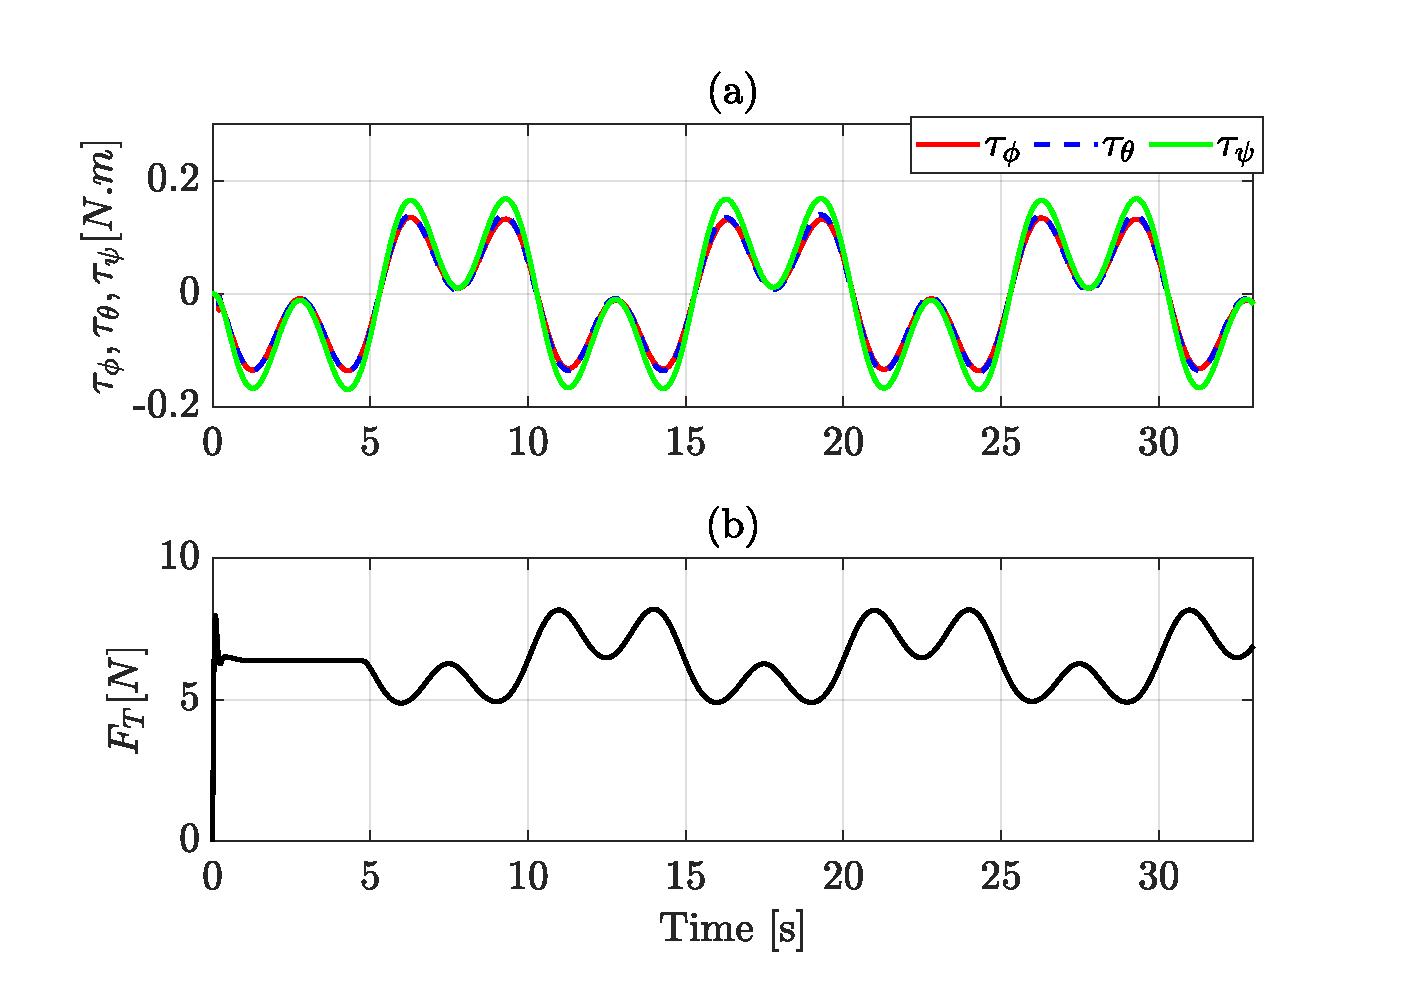
\includegraphics[width=14cm]{figure4/inputDisturbances.pdf}
    \caption{Control input signals under disturbance conditions: (a) angular torques $(\tau_\phi, \tau_\theta, \tau_\psi)$, (b) total thrust force ($F_T$). }
    \label{inputDisturbances}
\end{figure}

\subsection{Performance Evaluation under Combined Sensor and Actuator Faults}

To further assess the controller's robustness and fault tolerance, a challenging scenario involving simultaneous sensor and actuator faults was introduced at $t_f = 15s$. These faults included both additive and multiplicative components affecting the control inputs (angular torques and total thrust) and various sensors (angle, angular velocity, and linear speed sensors), while the position sensors were assumed to be fault-free. The specific characteristics and magnitudes of these faults are detailed in Table \ref{tab:faults}.

\begin{table}[h]
\centering
\caption{Actuator and sensor fault characteristics}
\label{tab:faults}
\begin{tabular}{lcc}
\hline
\textbf{Component} & \textbf{Additive Fault} & \textbf{Multiplicative Fault} \\
\hline
\hline
$\tau_\phi$, $\tau_\theta$ & $0.1 + 0.01t$ N$\cdot$m & $30\%$ \\
$\tau_\psi$ & $0.1 + 0.01t$ N$\cdot$m & $50\%$ \\
$F_T$ & $0.3 + 0.015t$ N & $50\%$ \\
$\phi$, $\theta$ & $0.01 + 0.005t$ rad & $30\%$ \\
$\psi$ & $0.15 + 0.01t$ rad & $30\%$ \\
$\dot{\phi}$, $\dot{\theta}$ & $0.1 + 0.01t$ rad/s & $30\%$ \\
$\dot{\psi}$ & $0.15 + 0.01t$ rad/s & $30\%$ \\
$\dot{p}_x$, $\dot{p}_y$& $0.3 + 0.02t$ m/s & $30\%$ \\
$\dot{p}_z$& $0.2 + 0.015t$ m/s & $50\%$\\
\hline
\end{tabular}
\end{table}

Fig.~\ref{attitudeWithFault} illustrates the attitude tracking response of the quadrotor under these severe fault conditions. While a degradation in tracking performance is observable after the faults are introduced at $t=15s$, particularly in the roll and pitch channels which exhibit increased deviations, the controller successfully maintains overall system stability. The yaw angle tracking also shows some deviation but remains controlled.

\begin{figure}[h!]
    \centering
    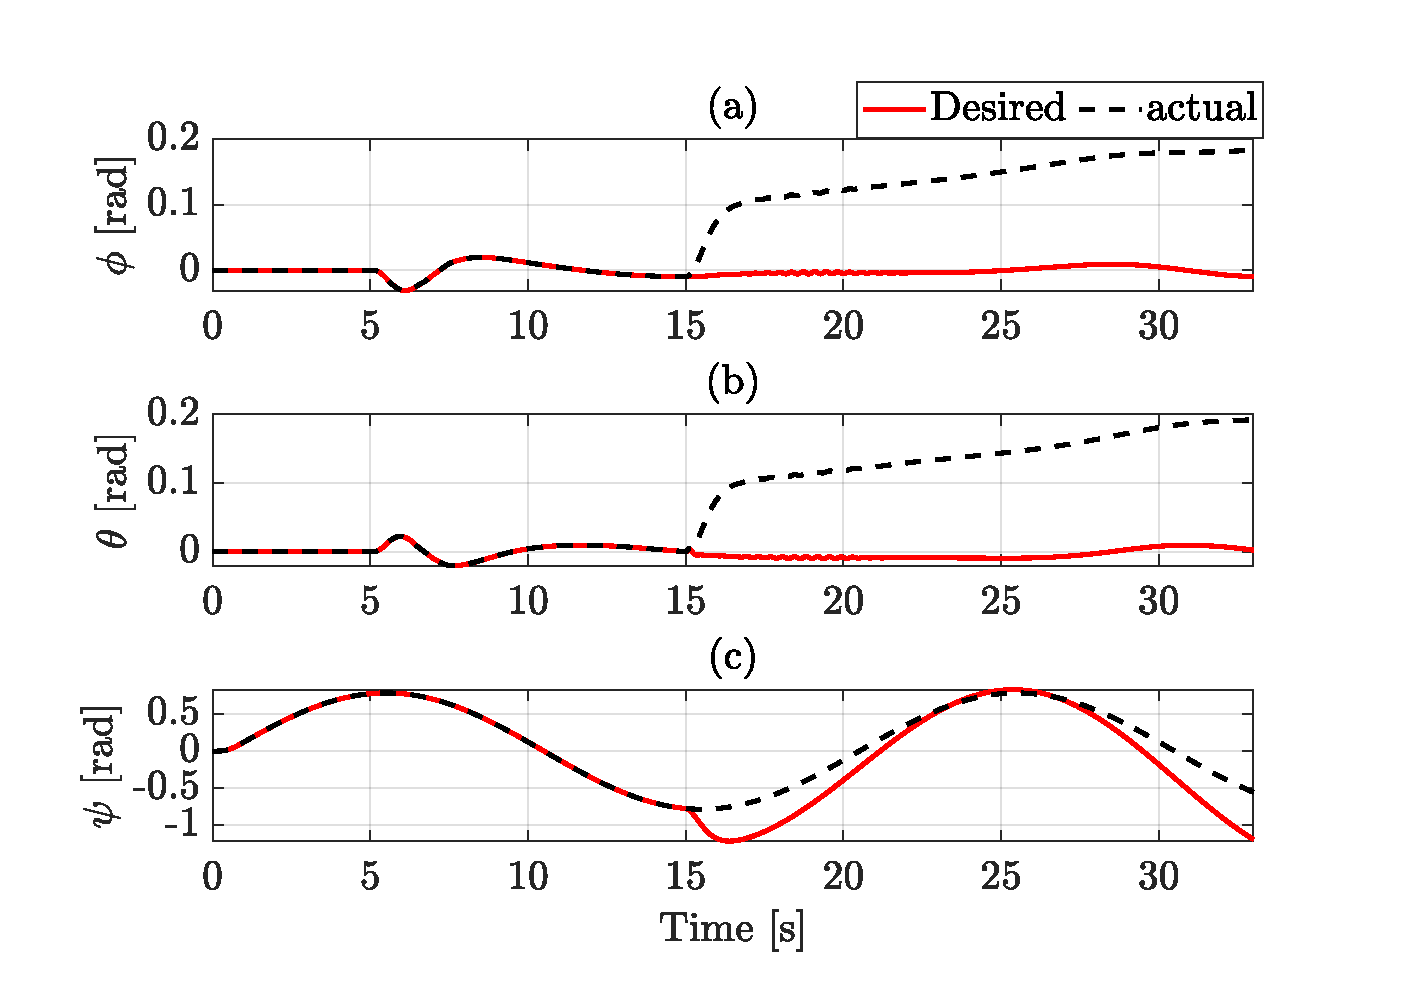
\includegraphics[width=14cm]{figure4/attitudeWithFault.pdf}
    \caption{Attitude tracking performance under combined actuator and sensor faults for: (a) roll ($\phi$), (b) pitch ($\theta$), and (c) yaw ($\psi$) angles. }
    \label{attitudeWithFault}
\end{figure}

The 3D trajectory tracking performance during this fault scenario is depicted in Fig.~\ref{3dFault}. This comparison again involves the PID controller (Set1), the non-optimized proposed controller (Set2), and the WOA-optimized proposed controller (Set3). Even with the compounded effects of sensor and actuator faults, the WOA-tuned controller (Set3) demonstrates superior fault-tolerant capabilities, maintaining a more stable flight path and better trajectory adherence compared to both the PID and the non-optimized controllers. This emphasizes the controller's ability to adapt to and mitigate the adverse effects of complex fault conditions.

\begin{figure}[h!]
    \centering
    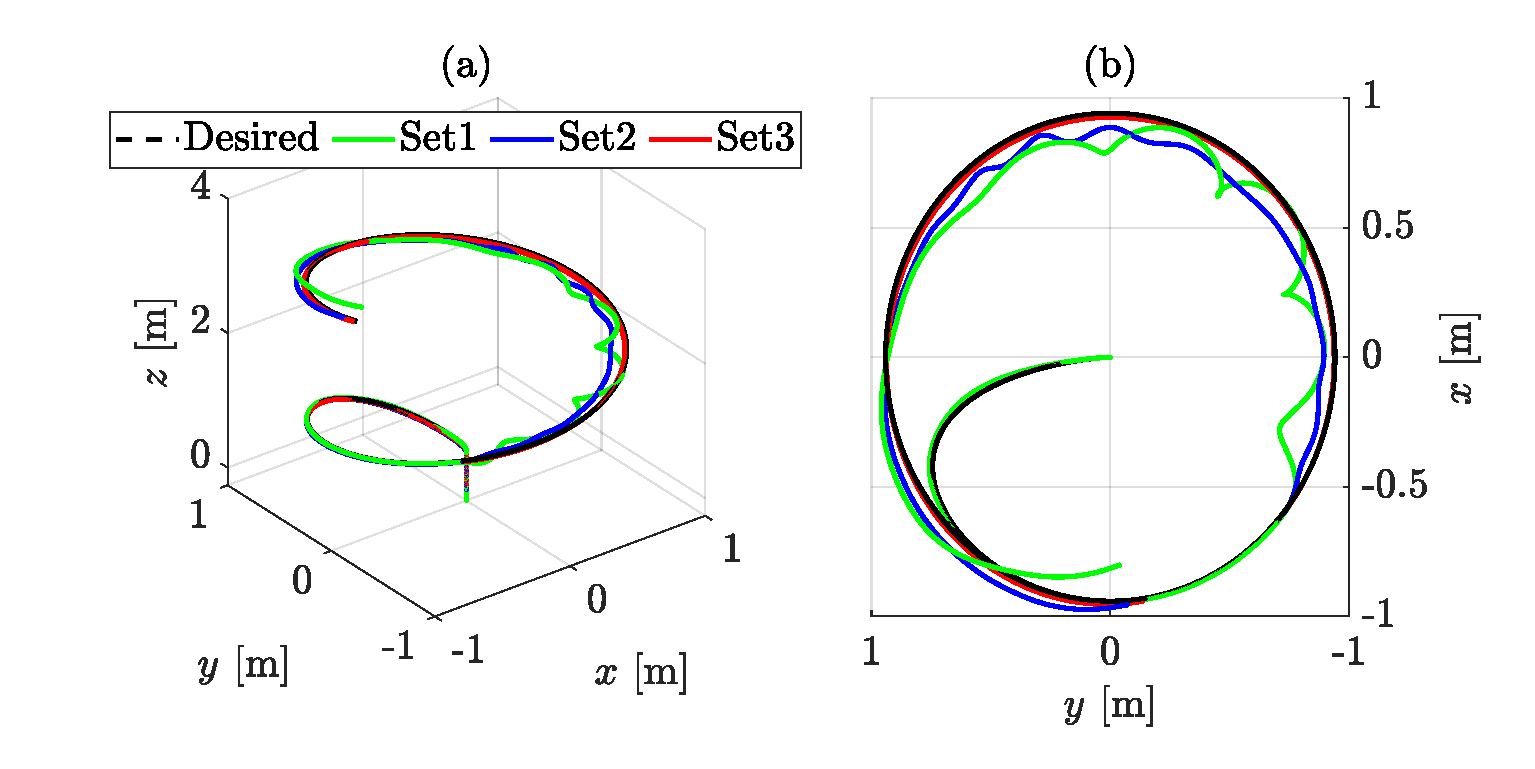
\includegraphics[width=14cm]{figure4/3dFault.pdf}
    \caption{3D trajectory tracking performance in fault conditions comparing PID, non-optimized, and WOA-optimized controllers: (a) side view, (b) top-down view. }
    \label{3dFault}
\end{figure}

The control inputs during the fault test are presented in Fig.~\ref{inputFault}. The angular torques show a distinct change in behavior after the fault injection at $t=15s$, followed by adjustments as the controller compensates for the fault effects. The total thrust force increases significantly, indicating the controller's effort to counteract the simulated loss of actuator effectiveness and maintain flight.

\begin{figure}[h!]
    \centering
    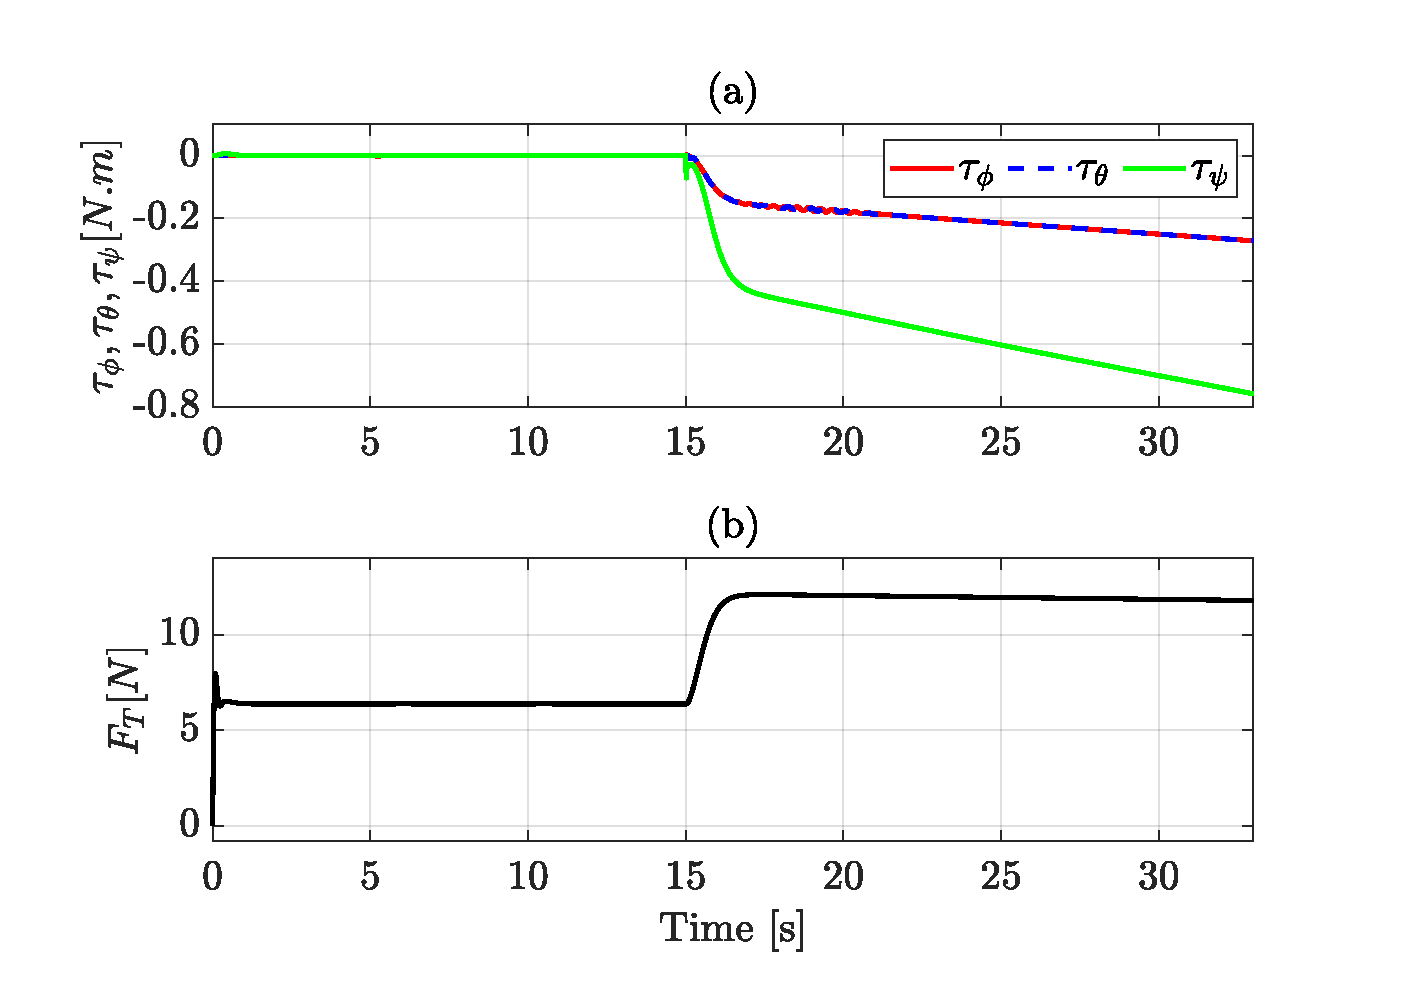
\includegraphics[width=14cm]{figure4/inputFault.pdf}
    \caption{Control signals in the presence of actuator and sensor faults: (a) angular torques $(\tau_\phi, \tau_\theta, \tau_\psi)$, (b) total thrust force ($F_T$). }
    \label{inputFault}
\end{figure}

\subsection{Overall Discussion}
The simulation studies comprehensively validate the proposed optimal fault-tolerant adaptive fuzzy control strategy for the quadrotor UAV. The controller demonstrates proficient trajectory tracking under nominal conditions with external disturbances and, more importantly, exhibits robust performance in the presence of complex, simultaneous sensor and actuator faults. The integration of the modified backstepping technique with fuzzy logic allows for effective adaptation to nonlinear dynamics, disturbances, and fault effects, while the fixed-time stability approach ensures rapid convergence. The application of the Whale Optimization Algorithm for parameter tuning proved crucial in achieving enhanced tracking accuracy and smoother control signals compared to manual tuning or other optimization methods like GWO, as demonstrated by the convergence curves in Fig. \ref{iterations}. The results suggest strong potential for the proposed control framework in real-world UAV applications where reliability and safety are paramount.

\begin{figure}
  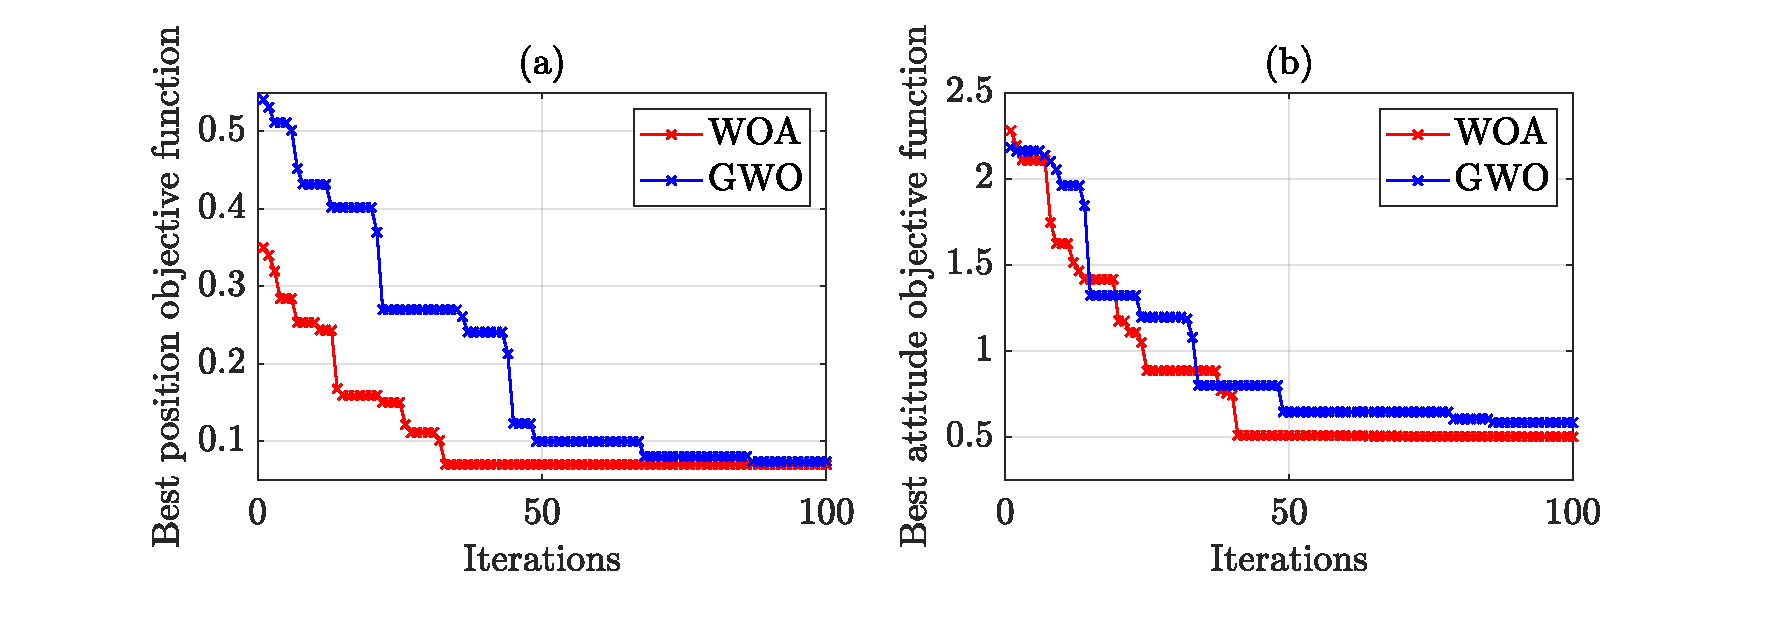
\includegraphics[width=14cm]{figure4/iterations_comparison.pdf}
  \caption{Comparison of convergence curves between WOA and GWO for (a) position control optimization and (b) attitude control optimization. }
      \label{iterations}
\end{figure}


\section{Summary}
\label{sec:conclusion_ch4}
In this chapter, an optimal fault-tolerant control strategy was developed for  a quadrotor UAV, addressing key challenges such as nonlinear dynamics, external disturbances, and potential sensor and actuator faults. The proposed solution is grounded in a combination of fixed-time stability theory, fuzzy logic inference systems, and the backstepping control technique, providing a robust and adaptive framework for ensuring reliable trajectory tracking under uncertain and faulty conditions.\\
The control strategy leverages fuzzy logic systems to approximate unknown nonlinear functions and disturbances in real-time, thereby eliminating the need for exact mathematical models. To ensure fast convergence and enhance resilience in time-sensitive UAV applications, the fixed-time control design guarantees stabilization within a predefined duration, regardless of the initial state.

Additionally, the WOA was integrated, which automatically tunes the controller's parameters to achieve optimal tracking accuracy and smooth control input signals. Compared to conventional methods such as PID control and manually tuned controllers, the proposed approach demonstrated superior performance in both fault-free and fault-induced scenarios.

In conclusion, the chapter introduced a practical and high-performance fault-tolerant control framework suitable for real-time quadrotor UAV operations, with potential for future application in multi-UAV systems and experimental validation on physical platforms.